%=====================================================================

\chapter{Using Tabling in XSB: A Tutorial Introduction} 
\label{chap:TablingOverview}

XSB has two ways of evaluating predicates.  The default is to use
Prolog-style evaluation, but by using various declarations a
programmer can also use tabled resolution which can provide a
different, more declarative programming style than Prolog.  In this
section we discuss various aspects of tabling and its implementation
in XSB\@.  Our aim in this section is to provide a user with enough
information to be able to program productively with tables in XSB\@.
It is best to read this tutorial with a copy of XSB handy, since much
of the information is presented through a series of exercises.

For the theoretically inclined, XSB uses SLG resolution which can
compute queries to non-floundering normal programs under the
well-founded semantics~\cite{VGRS91}, and is guaranteed to terminate
when these programs have the {\em bounded term-depth property}.  This
tutorial covers only enough of the theory of tabling to explain how to
program in XSB\@.  For those interested, the web site contains papers
covering in detail various aspects of tabling (often through the links
for individuals involved in XSB)\@.  An overview of SLG resolution,
and practical evaluation strategies for it, are provided
in~\cite{ChWa96,Swif99b,SaSW99,FSW98}.  The engine of XSB, the
SLG-WAM, is an extension of the WAM \cite{DHWa83,AitK90}, and is
described in~\cite{SaSw98,RRSSW98,JFLP-Scheduling,SaSW96,
ChSW95,CAT@PLILP-98,TST99,CuSW99b,CaSW02} as it is implemented in
\version{} and its performance analyzed. Examples of large-scale
applications that use tabling are overviewed in~\cite{syntactica,
semantica, CoDS96, DRW96, RRRSSW97, Boul97,CuSW99a,GSTPD00}.

%=====================================================================

\section{XSB as a Prolog System}
\label{tabling_env}

Before describing how to program using tabling it is perhaps
worthwhile to review some of the goals of XSB's implementation of
tabling*.  Among them are:
\begin{enumerate}
\item	To execute tabled predicates at the speed of compiled Prolog.
\item	To ensure that the speed of compiled Prolog is not slowed
	significantly by adding the option of tabling.
\item	To ensure that the functionality of Prolog is not compromised
 	by support for tabling.
\item   To provide Prolog functionality in tabled predicates and
	operators whenever it is semantically sensible to do so.
\item	To provide standard predicates to manipulate tables
	taken as data structures in themselves.
\end{enumerate}

Goals 1 and 2 are addressed by XSB's engine, which in \version{} is
based on a virtual machine called the SLG-WAM\@.  The overhead for SLD
resolution using this machine is small, and usually less than 5\%.
Thus when XSB is used simply as a Prolog system (i.e., no tabling is
used), it is reasonably competitive with other Prolog implementations
based on a WAM emulator written in C or assembly.  For example, when
compiled as a threaded interpreter (see Chapter~\ref{system}) XSB
\version\ is about two times slower than Quintus 3.1.1 or emulated
SICStus Prolog 3.1.
%
Goals 3, 4 and 5 have been nearly met, but there are a few instances
in which interaction of tabling with a Prolog construct has not been
accomplished, or is perhaps impossible.  Accordingly we discuss these
instances throughout this chapter.  XSB is still under development
however, so that future versions may support more transparent mixing
of Prolog and tabled code.
\comment{
 (e.g. allowing tabled predicates in the
scope of \verb|\+/1|) or adding Prolog functionality to tabled
predicates or operators (e.g. allowing non-ground negation in {\tt
tnot/1}).
}
%=====================================================================

\section{Definite Programs}
\label{sec:def}

Definite programs, also called \emph{Horn Clause Programs}, are Prolog
programs without negation or aggregation.  In XSB, this means without
the \verb|\+/1|, {\tt fail\_if/1}, {\tt not/1}, {\tt tnot/1} or aggregation 
operators.  Consider the Prolog program
\begin{center}
\begin{minipage}{3.8in}
\begin{verbatim}
path(X,Y) :- path(X,Z), edge(Z,Y).
path(X,Y) :- edge(X,Y).
\end{verbatim}						       
\end{minipage}
\end{center}
together with the query {\tt ?- path(1,Y)}.  This program has a
simple, declarative meaning: there is a path from {\tt X} to {\tt Y}
if there is a path from {\tt X} to some node {\tt Z} and there is an
edge from {\tt Z} to {\tt Y}, or if there is an edge from {\tt X} to
{\tt Y}\@.  Prolog, however, enters into an infinite loop when
computing an answer to this query.  The inability of Prolog to answer
such queries, which arise frequently, comprises one of its major
limitations as an implementation of logic.

A number of approaches have been developed to address this problem by
reusing partial answers to the query {\tt path(1,Y)}
\cite{Diet87,TaSa86,BMSU86,Viei89,Walk93}.  The ideas behind these
algorithms can be described in the following manner.  Calls to tabled
predicates, such as {\tt path(1,Y)} in the above example, are stored
in a searchable structure together with their proven instances.  This
collection of \emph{tabled subgoals} paired with their \emph{answers},
generally referred to as a \emph{table}, is consulted whenever a new
call, $C$, to a tabled predicate is issued.  If $C$ is sufficiently
similar to a tabled subgoal $S$, then the set of answers, $\cA$,
associated with $S$ may be used to satisfy $C$.
%\footnote{We use
%the term ``answer set'' to describe the set of answers associated with
%a given subgoal during a given state of computation.  As such, it has
%no relation to the use of the term ``answer set'' in the non-monotonic
%literature.}\@.  
In such instances, $C$ is resolved against the answers in $\cA$, and
hence we refer to $C$ as a \emph{consumer}\index{tabling!consumer} of
$\cA$ (or $S$)\@.  If there is no such $S$, then $C$ is entered into
the table and is resolved against program clauses as in
Prolog~---~i.e., using SLD~resolution.  As each answer is derived
during this process, it is inserted into the table entry associated
with $C$ if it contains information not already in $\cA$\@.  We hence
refer to $C$ as a \emph{generator}, or
\emph{producer}\index{tabling!producer, generator}, as resolution of
$C$ in this manner produces the answers stored in its table entry.  If
the answer is in fact added to this set, then it is additionally
scheduled to be returned to all consumers of $C$\@.  If instead it is
rejected as redundant, then the evaluation simply fails and backtracks
to generate more answers.

Notice that since consuming subgoals resolve against unique answers
rather than repeatedly against program clauses, tabling will terminate
whenever
\begin{enumerate}
\item a finite number of subgoals are encountered during query
      evaluation, and
\item each of these subgoals has a finite number of answers.
\end{enumerate}
Indeed, it can be proven that for any program with the \emph{bounded
term depth property}~---~roughly, where all terms generated in a
program have a maximum depth~---~SLG computation will terminate.
These programs include the important class of \emph{Datalog} programs.

%--------------------------------------------------------------------
Predicates can be declared tabled in a variety of ways.  A common form
is the compiler directive \stdrefindex{table/1}
\[
	\verb|:- table | P_1, \ldots, P_n.
\]
where $P_i$ is a predicate indicator or callable term.  More
generally as explained below,
\[
	\verb|:- table | P_1, \ldots, P_n\ {\tt as\ Options}.
\]
allows a user to specify different types of tabling through {\tt
  Options} along with other properties of the designated predicates
For static predicates, these directives must be added to the file
containing the clauses of the predicate(s) to be tabled, and compiles
them to use tabling~\footnote{In \version, tabling does not work
  together with multi-file predicates.}.  For dynamic predicates, the
executable directive
\[
       \verb| ?- table | p/n.
\]
causes {\tt p/n} to be tabled if no clauses have been asserted for
{\tt p/n}.

\paragraph{Exercises}
Unless otherwise noted, the file
\textup{\texttt{\$XSB\_DIR/examples/table\_examples.P}} contains all
the code for the running examples in this section.  Invoke XSB with its
default settings (i.e., don't supply additional options) when working
through the following exercises.

\begin{exercise}
Consult \textup{\texttt{\$XSB\_DIR/examples/table\_examples.P}} into
XSB and and try the goal
\begin{verbatim}
         ?- path(1,X).
\end{verbatim}
and continue typing \verb|;<RETURN>| until you have exhausted all
answers.  Now, try rewriting the \code{path/2} predicate as it would
be written in Prolog~---~and without a tabling declaration.  Will it
now terminate for the provided {\tt edge/2} relation?  (Remember, in
XSB you can always hit \verb|<ctrl>-C| if you go into an infinite
loop).\fillBox
\end{exercise}

The return of answers in tabling aids in filtering out redundant
computations -- indeed it is this property which makes tabling
terminate for many classes of programs.  The {\em same generation}
program furnishes a case of the usefulness of tabling for optimizing a
Prolog program.

\begin{exercise} \label{ex:samegen}
If you are {\em still} curious, load in the file {\tt cyl.P} in the
\verb|$XSB_DIR/examples| directory using the command.
\begin{verbatim}
         ?- load_dync(cyl.P).
\end{verbatim}
and then type the query
\begin{verbatim}
         ?- same_generation(X,X),fail.
\end{verbatim}
Now rewrite the {\tt same\_generation/2} program so that it does not
use tabling and retry the same query.  What happens?  (Be
patient~---~or use \verb|<ctrl>-C|).\fillBox
\end{exercise}

\begin{exercise}
The file {\tt table\_examples.P} contains a set of facts
\begin{verbatim}
         ordered_goal(one).
         ordered_goal(two).
         ordered_goal(three).
         ordered_goal(four).
\end{verbatim}
Clearly, the query {\tt ?- ordered\_goal(X)} will return the answers
in the expected order.  {\tt table\_examples.P} also contains a predicate
\begin{verbatim}
         :- table table_ordered_goal/1.
         table_ordered_goal(X):- ordered_goal(X).
\end{verbatim}
which simply calls {\tt ordered\_goal/1} and tables its answers
(tabling is unnecessary in this case, and is only used for
illustration).  Call the query {\tt ?- table\_ordered\_goal(X)} and
backtrack through the answers.  In what order are the answers
returned?
\end{exercise}
%-------------------------------------------------------------------------
\comment{
\begin{exercise}
Consult this file into XSB and type the query
\begin{verbatim}
         ?- path(1,Y).
\end{verbatim}
and continue typing \verb|;<RETURN>| until you have exhausted all
answers.  Type the query again.  Can you guess why the order of
answers is different?  Now type
\begin{verbatim}
         ?- abolish_all_tables.
\end{verbatim}
and retry the \code{path/2} query.\fillBox
\end{exercise}
}
%-------------------------------------------------------------------------

The examples stress two differences between tabling and SLD resolution
beyond termination properties.  First, that each solution to a tabled
subgoal is returned only once~---~a property that is helpful not only
for {\tt path/2} but also for {\tt same\_generation/2} which
terminates in Prolog.  Second, because answers are sometimes obtained
using program clauses and sometimes using the table, answers may be
returned in an unaccustomed order.

\paragraph*{Tabling Dynamic Predicates}

Dynamic predicates may be tabled just as static predicates, as the
following exercise shows.

\begin{exercise}
For instance, restart XSB and at the prompt type the directive
\begin{verbatim}
         ?- table(dyn_path/2).
\end{verbatim}
and 
\begin{verbatim}
         ?- load_dyn(dyn_examples).
\end{verbatim}
Try the queries to {\tt path/2} of the previous examples.  Note that
it is important to dynamically load {\tt dyn\_examples.P} ---
otherwise the code in the file will be compiled without knowledge of
the tabling declaration.\fillBox
\end{exercise}

In general, as long as the directive {\tt table/1} is executed before
asserting (or dynamically loading) the predicates referred to in the
directive, any dynamic predicate can be tabled.

\paragraph*{Letting XSB Decide What to Table}
Other tabling declarations are also provided.  Often it is tedious to
decide which predicates must be tabled.  To address this, XSB can
automatically table predicates in files.  The declaration {\tt
  auto\_table}\index{declarations!\texttt{auto\_table}} chooses predicates to table
to assist in termination, while {\tt
  suppl\_table}\index{declarations!\texttt{suppl\_table}} chooses predicates to
table to optimize data-oriented queries.  Both are explained in
\refsec{sec:CompilerOptions}.~\footnote{The reader may have noted that
  {\tt table/1}, is referred to as a \emph{directive}, while {\tt
    auto\_table/0} and {\tt suppl\_table/0} were referred to as
  \emph{declarations}.  The difference is that at the command line,
  user can execute a directive but not a compiler declaration.}.

%--------------------------------------------------------------------

\subsection{Call Variance vs. Call Subsumption}
\label{sec:SimilarityMeasures}
\index{tabling!similarity measures}

The above description gives a general characterization of tabled
evaluation for definite programs but glosses over certain details.  In
particular, we have not specified the criteria for 
\begin{itemize}
\item {\em Call Similarity} -- whereby a newly issued call $C$ is
  determined to be ``sufficiently similar'' to a tabled subgoal $S$ so
  that $C$ can use the answers from the table of $S$ rather than
  re-deriving its own answers.  In the first case where $C$ uses
  answers of a tabled subgoal it is termed a consumer; in the second
  case when $C$ produces its own answers it is called a generator.
%
\item {\em Answer Similarity} -- whereby a derived answer to a tabled
  subgoal is determined to contain information similar to that already
  in the set of answers for that subgoal.
\end{itemize}
Different measures of similarity are possible.  XSB's engine supports
two measures for call similarity: variance and subsumption.  XSB's
engine supports a variance-based measure for answer similarity, but
allows users to program other measures in certain cases.  We discuss
call similarity here, but defer the discussion of answer similarity
until Section~\ref{sec:table-aggregation}).

% - - - - - - - - - - - - - - - - - - - - - - - - - - - - - - - - - -

\paragraph{Determining Call Similarity via Variance}
\index{tabling!variant-based} 
%
By default, XSB determines that a call $C$ is similar to a tabled
subgoal $S$ if $C$ is a variant of $S$~---~\footnote{Formally, $C$ and
  $S$ are variants if there are substitutions $\theta_1$ and
  $\theta_2$ such that the ranges of $\theta_1$ and $\theta_2$ consist
  only of variables, and $C\theta_1 = S$, and $S\theta_2 = C$.}.  As
an example {\tt p(X,Y,X)} is a variant of {\tt p(A,B,A)}, but not of
{\tt p(X,Y,Y)}, or {\tt p(X,Y,Z)}.  Variance-based call similarity
was used in the original formulation of SLG resolution \cite{ChWa96}
for the evaluation of normal logic programs according to the
well-founded semantics and interacts well with many of Prolog's
extra-logical constructs.

Under variance-based call similarity, when a tabled call $C$ is made,
a search for a table entry containing a variant subgoal $S$ is
performed.  Notice that if such an $S$ should exist, then \emph{all}
of its answers are also answers to $C$, and therefore will be resolved
against it.  
\comment{
Likewise, when an answer $A$ is derived for a producing
subgoal $S$, $A$ is inserted into the answer set $\cA$ of $S$ if and
only if $A$ does not already exist in $\cA$~---~that is, if there is
no variant of $A$ already present in $\cA$\@.  The insertion of $A$,
therefore, leads to the return of $A$ to consumers of $S$\@.  However,
the return of only the most general answers to a consumer, referred to
as \emph{answer subsumption}, can be flexibly programmed as discussed
in Section~{\ref{sec:table-aggregation}}
}

% - - - - - - - - - - - - - - - - - - - - - - - - - - - - - - - - - -

\paragraph{Determining Call Similarity via Subsumption}
\index{tabling!call subsumption-based}

Call similarity can also be based on subsumption.  A term $T_1$
\emph{subsumes} a term $T_2$ if $T_2$ is more specific than
$T_1$~\footnote{Formally, $T_1$ subsumes $T_2$ if there is a
  substitution $\theta$ whose domain consists only of variables from
  $T_1$ such that $T_1\theta = T_2$.}.  Furthermore, we say that $T_1$
\emph{properly subsumes} $T_2$ if $T_2$ is not a variant of $T_1$.
Under subsumption-based tabling, when a tabled call $C$ is issued, a
search is performed for a table entry containing a subsuming subgoal
$S$\@.  Notice that, if such an entry exists, then its answer set
$\cA$ logically contains all the solutions to satisfy $C$\@.  The
subset of answers $\cA' \subseteq \cA$ which unify with $C$ are said
to be \emph{relevant to} $C$\@.  Likewise, upon the derivation of an
answer $A$ for a producing subgoal $S$, $A$ is inserted into the
answer set $\cA$ of $S$ if and only if $A$ is not subsumed by some
answer $A'$ already present in $\cA$\@.

Notice that subsumption-based tabling permits greater reuse of
computed results, thus avoiding even more program resolution, and
thereby can lead to time and space performances superior to
variant-based tabling.  In addition, beginning with Version 3.2,
call-subsumption based tabling fully supports well-founded negation
under the default local scheduling strategy.  However, there are
downsides to this paradigm.  First of all, subsumptively tabled
predicates do not interact well with certain Prolog constructs with
which variant-tabled predicates can (see
Example~\ref{example:sub-fail} below).  Second, call subsumption does
not yet support calls with tabled attributed variables or answer
subsumption~\footnote{Beginning with Version 3.2, XSB supports
  attributed variables in answers under call subsumption, although not
  in calls.}.

%Further, in the
%current implementation of subsumption-based tabling, subsumptive
%predicates may not take part in negative computations which result in
%the \emph{delay} \index{tabling!call subsumption-based!interaction with
%  negation} of a literal containing a subsumptive subgoal (see
%\refsec{sec:CurrentRestrictions}).  This requires subcomputations in
%which subsumptive predicates take part to be LRD-stratified (see
%Section~\ref{sec:lrd}).

\begin{example}
The terms $T_1$: {\tt p(f(Y),X,1)} and $T_2$:~{\tt p(f(Z),U,1)} are
\emph{variants} as one can be made to look like the other by a
renaming of the variables.  Therefore, each \emph{subsumes} the other. \\
\noindent The term $t_3$: {\tt p(f(Y),X,1)} \emph{subsumes} the term
$t_4$:~{\tt p(f(Z),Z,1)}.  However, they are \emph{not variants}.  Hence
$t_3$ \emph{properly subsumes}~$t_4$.\fillBox
\end{example}

The above examples show how a variant-based tabled evaluation can
reduce certain redundant subcomputations over SLD\@.  However, even
more redundancy can be eliminated, as the following example shows.

\begin{exercise} \label{ex:VarVsSub}
Begin by abolishing all tables in XSB, and then type the following query
\begin{verbatim}
         ?- abolish_all_tables.
         ?- path(X,Y), fail.
\end{verbatim}
Notice that only a single table entry is created during the evaluation
of this query.  You can check that this is the case by invoking the
following query
\begin{verbatim}
         ?- get_calls_for_table(path/2,Call).
\end{verbatim}
Now evaluate the query
\begin{verbatim}
         ?- path(1,5), fail.
\end{verbatim}
and again check the subgoals in the table.  Notice that two more have
been added.  Further notice that these new subgoals are
\emph{subsumed} by that of the original entry.  Correspondingly, the
answers derived for these newer subgoals are already present in the
original entry.  You can check the answers contained in a table entry
by invoking \code{get\_returns\_for\_call/2} on a tabled subgoal.  For
example:
\begin{verbatim}
         ?- get_returns_for_call(p(1,_),Answer).
\end{verbatim}
Compare these answers to those of \code{p(X,Y)} and \code{p(1,5)}.
Notice that the same answer can, and in this case does, appear in
multiple table entries.

Now, let's again abolish all the tables and change the evaluation
strategy of \code{path/2} to use subsumption.
\begin{verbatim}
	 ?- abolish_all_tables.
         ?- use_subsumptive_tabling path/2.
\end{verbatim}
And re-perform the first few queries:
\begin{verbatim}
         ?- path(X,Y),fail.
	 ?- get_calls_for_table(path/2,Call).
	 ?- path(1,5).
	 ?- get_calls_for_table(path/2,Call).
\end{verbatim}
Notice that this time the table has not changed!  Only a single entry
is present, that for the original query \code{p(X,Y)}.
\end{exercise}
%
When using subsumption-based tabling, XSB is able to recognize a greater
range of ``redundant'' queries and thereby make greater use of
previously computed answers.  The result is that less program resolution
is performed and less redundancy is present in the table.  However,
subsumption is not a panacea.  The elimination of redundant answers
depends upon the presence of a subsuming subgoal in the table when the
call to \code{p(1,5)} is made.  If the order of these queries were
reversed, one would find that the same entries would be present in this
table as the one constructed under variant-based evaluation.

\paragraph{Declarations for Call Variance and Call Subsumption}
By default tabled predicate use call variance.  However,
subsumption-based tabling can be made the default by giving XSB the
\verb|-S| option at invocation (refer to \refsec{sec:EmuOptions}).
More versatile constructs are provided by XSB so that the tabling
method can be selected on a \emph{per predicate} basis.  Use of either
directive
\texttt{use\_variant\_tabling/1}\index{declarations!\texttt{use\_variant\_tabling/1}}
or
\texttt{use\_subsumptive\_tabling/1},\index{declarations!\texttt{use\_subsumptive\_tabling/1}}
described in \refsec{sec:TablePred:Decl&Mod}, ensures that a tabled
predicate is evaluated using the desired strategy regardless of the
default tabling strategy.

%----------------------------------------------------------------------

\subsection{Table Scheduling Strategies} \label{section:scheduling}
\index{tabling!scheduling strategies}
�
Recall that SLD resolution works by selecting a goal from a list of
goals to be proved, and selecting a program clause $C$ to resolve
against that goal.  During resolution of a top level goal $G$, if the
list of unresolved goals becomes empty, $G$ succeeds, while if there
is no program clause to resolve against the selected goal from the
list resolution against $G$ fails.  In Prolog clauses are selected in
the order they are asserted, while literals are selected in a
left-to-right selection strategy.  Other strategies are possible for
SLD, and in fact completeness of SLD for definite programs depends on
a non-fixed literal selection strategy.  This is why Prolog, which has
a fixed literal selection strategy is not complete for definite
programs, even when they have bounded term-depth.

Because tabling uses program clause resolution, the two parameters of
clause selection and literal selection also apply to tabling.  Tabling
makes use of a dynamic literal selection strategy for certain
non-stratified programs (via the delaying mechanism described in
Section~\ref{negation!unstratified}), but uses the same left-to-right
literal selection strategy as Prolog for definite programs.  However,
in tabling there is also a choice of when to return derived answers to
subgoals that consume these answers.  While full discussion of
scheduling strategies for tabling is not covered here
(see~\cite{JFLP-Scheduling}) we discuss two scheduling strategies
that have been implemented for XSB \version~\footnote{Many other
  scheduling strategies are possible.  For instance, \cite{FrSW97}
  describes a tabling strategy implemented for the SLG-WAM that
  emulates magic sets under semi-naive evaluation.  This scheduling
  strategy, however, is not available in \version{} of XSB.}.

\begin{itemize}

\item {\em Local Scheduling} Local Scheduling depends on the notion of
  a {\em subgoal dependency graph}.  For the state of a tabled
  evaluation, a non-completed tabled subgoal $S_1$ directly depends on
  a non-completed subgoal $S_2$ when $S_2$ is in the SLG tree for
  $S_1$ -- that is when $S_2$ is called by $S_1$ without any
  intervening tabled predicate.  The edges of the subgoal dependency
  graph are then these direct dependency relations, so that the
  subgoal dependency graph is directed.  As mentioned, the subgoal
  dependency graph reflects a given state of a tabled evaluation and
  so may changed as the evaluation proceeds, as new tabled subgoals
  are encountered, or encountered in different contexts, as tables
  complete, and so on.  As with any directed graph, the subgoal
  dependency graph can be divided up into strongly connected
  components, consisting of tabled subgoals that depend on one
  another.  Local scheduling then fully evaluates each maximal SCC (a
  SCC that does not depend on another SCC) before returning answers to
  any subgoal outside of the SCC~\footnote{XSB's implementation
    maintains a slight over-approximation of SCCs -- see
    \cite{JFLP-Scheduling}.}.

\item {\em Batched Scheduling} Unlike Local Scheduling, Batched
  Scheduling allows answers to be returned outside of a maximal SCC as
  they are derived, and thus resembles Prolog's tuple at a time
  scheduling.  
\end{itemize}

Both Local and Batched Scheduling have their advantages, and we list
points of comparison.

\begin{itemize}

\item {\em Time for left recursion} Batched Scheduling is somewhat
  faster than Local Scheduling for left recursion as Local Scheduling
  imposes overhead to prevent answers from being returned outside of
  a maximal SCC.  

\item {\em Time to first answer}  Because Batched Scheduling returns
  answers out of an SCC eagerly, it is faster to derive the first
  answer to a tabled predicate.

\item {\em Stack space} Local evaluation generally requires less space
  than batched evaluation as it fully explores a maximal SCC,
  completes the SCC's subgoals, reclaims space, and then moves on to a
  new SCC.  

\item {\em Integration with cuts} As discussed in
  Exercise~\ref{ex:nocut} and throughout Section~\ref{sec:cuts}, Local
  Scheduling integrates better with cuts, although this is partly
  because tabled subgoals may be fully evaluated before the cut takes
  effect. 

\item {\em Efficiency for call subsumption} Because Local Evaluation
  completes tables earlier than Batched Evaluation it may be faster
  for some uses of call subsumption, as subsumed calls can make use of
  completed subsuming tables.

\item {\em Negation and tabled aggregation} As will be shown below,
  Local Scheduling is superior for tabled aggregation as only optimal
  answers are returned out of a maximal SCC.  Local Scheduling also
  can be more efficient for non-stratified negation as it may allow
  delayed answers that are later simplified away to avoid being
  propagated.
\end{itemize}

On the whole, advantages of Local Scheduling outweigh the advantages of
Batched Scheduling, and for this reason Local Scheduling is the
default scheduling strategy for \version{} of XSB.  XSB can be
configured to use batched scheduling via the configuration option {\tt
  --enable-batched-scheduling} and remaking XSB\@.  This will not
affect the default version of XSB, which will also remain available.

%--------------------------------------------------------------------

\subsection{Interaction Between Prolog Constructs and Tabling}

Tabling integrates well with most non-pure aspects of Prolog.
Predicates with side-effects like {\tt read/1} and {\tt write/1} can
be used freely in tabled predicates as long as it is remembered that
only the first call to a goal will execute program clauses while the
rest will look up answers from a table.  However, other extra-logical
constructs like the cut (\texttt{!}) pose greater difficulties.
Subsumption-based tabling is also theoretically precluded from correct
interaction with certain meta-logical predicates.

\paragraph{Cuts and Tabling} \label{sec:cuts}
\index{tabling!cuts}

The semantics for cuts in Prolog is largely operational, and is
usually defined based on an ordered traversal of an SLD search tree.
Tabling, of course, has a different operational semantics than Prolog
-- it uses SLG trees rather than SLD trees, for instance -- so it is
not surprising that the interaction of tabling with cuts is
operational.  In Prolog, the semantics for a cut can be expressed in
the following manner: a cut executed in the body of a predicate $P$
frames from the top (youngest end) of the choice point stack down to
and including the call for $P$.  In XSB {\em a cut is allowed to
  succeed as long as it does not cut over a choice point for a
  non-completed tabled subgoal, otherwise, the computation aborts}.
This means, among other matters, that the validity of a cut depends on
the {\em scheduling strategy} used for tabling, that is on the
strategy used to determine when an answer is to be returned to a
consuming subgoal.  Scheduling strategy was discussed
Section~\ref{section:scheduling}: for now, we assume that XSB's
default local scheduling is used in the examples for cuts.

\begin{exercise} \label{ex:nocut}
Consider the program
\begin{verbatim}
:- table cut_p/1, cut_q/1, cut_r/0, cut_s/0.

cut_p(X) :- cut_q(X), cut_r.
cut_r :- cut_s.
cut_s :- cut_q(_).
cut_q(1).   cut_q(2).
\end{verbatim}
What solutions are derived for the goal {\tt ?- cut\_p(X)}\@?  Suppose
that {\tt cut\_p/1} were rewritten as
\begin{verbatim}
cut_p(X) :- cut_q(X), once(cut_r).
\end{verbatim}
How should this cut over a table affect the answers generated for {\tt
cut\_p/1}?  What happens if you rewrite {\tt cut\_p/1} in this way and
compile it in XSB?\fillBox
\end{exercise}

In Exercise \ref{ex:nocut}, {\tt cut\_p(1)} and {\tt cut\_p(2)} should
both be true.  Thus, the cut in the literal {\tt once(cut\_r)} must
not inadvertently cut away solutions that are demanded by {\tt
  cut\_p/1}.  In the default local scheduling of XSB \version{} tabled
subgoals are fully evaluated whenever possible before returning any of
their answers.  Thus the first call {\tt cut\_q(X)} in the body of the
clause for {\tt cut\_p/1} is fully evaluated before proceeding to the
goal {\tt once(cut\_r)}.  Because of this any choice points for {\tt
  cut\_q(X)} are to a completed table.  For other scheduling
strategies, such as batched scheduling, non-completed choice points
for {\tt cut\_p/1} may be present on the choice point stack so that the
cut would be disallowed.  In addition, it is also possible to
construct examples where a cut is allowed if call variance is used,
but not if call subsumption is used.

\begin{example}
A further example of using cuts in a tabled predicate is a tabled
meta-interpreter.
\begin{verbatim}
:- table demo/1.

demo(true).
demo((A,B)) :- !, demo(A), demo(B).
demo(C) :- call(C).
\end{verbatim}
More elaborate tabled meta-interpreters can be extremely useful, for
instance to implement various extensions of definite or normal
programs.\fillBox
\end{example}

In XSB's compilation, the cut above is compiled so that it is valid to
use with either local or batched (a non-default) evaluation.  An
example of a cut that is valid neither in batched nor in local
evaluation is as follows.

\begin{example} \label{ex:cutTable}
Consider the program
\begin{verbatim}
:- table cut_a/1, cut_b/1.

cut_a(X):- cut_b(X).
cut_a(a1).

cut_b(X):- cut_a(X).
cut_b(b1).
\end{verbatim}
For this program the goal {\tt ?- cut\_a(X)} produces two answers, as
expected: {\tt a1} and {\tt b1}.  However, replacing the first class
of the above program with 
\begin{verbatim}
cut_a(X):- once(cut_b(X)).
\end{verbatim}
will abort both in batched or in local evaluation.
\fillBox
\end{example}

To summarize, the behavior of cuts with tables depends on dynamic
operational properties, and we have seen examples of programs in which
a cut is valid in both local and batched scheduling, in local but not
batched scheduling, and in neither batched nor local scheduling.  In
general, any program and goal that allows cuts in batched scheduling
will allow them in local scheduling as well, and there are programs
for which cuts are allowed in local scheduling but not in batched.

Finally, we note that in \version{} of XSB a ``cut'' over tables
implicitly occurs when the user makes a call to a tabled predicate
from the interpreter level, but does not generate all solutions.  This
commonly occurs in batched scheduling, but can also occur in local
scheduling if an exception occurs.  In such a case, the user will see
the warning {\tt "Removing incomplete tables..."} appear.  Any
complete tables will not be removed.  They can be abolished by using
one of XSB's predicates for abolishing tables.

\paragraph{Subsumption-Based Tabling and Meta-Logical Predicates}
\index{tabling!call subsumption-based!interaction with meta-logical predicates}

Meta-logical predicates like {\tt var/1} can be used to alter the
choices made during an evaluation.  However, this is dangerous when
used in conjunction with a paradigm that assumes that if a specific
relation holds~---~e.g., \texttt{p(a)}~---~then a more general
query~---~e.g., \texttt{p(X)}~---~will reveal this fact.

\begin{example}\label{example:sub-fail}
Consider the following simple program
\begin{verbatim}
        p(X) :- var(X), X = a.
\end{verbatim}
to which the queries
\begin{verbatim}
        ?- p(X).
        ?- p(a).
\end{verbatim}
are posed.  Let us compare the outcome of these queries when
\code{p/1} is (1)~a Prolog predicate, (2)~a variant-tabled predicate,
and (3)~a subsumptive-tabled predicate.

Both Prolog and variant-based tabling yield the same solutions: \code{X
= a}\, and\, \code{no}, respectively.  Under subsumption-based tabling,
the query \verb|?-|$\;$\code{p(X).} likewise results in the solution
\code{X = a}.  However, the query \verb|?-|$\;$\code{p(a).}  is subsumed
by the tabled subgoal \code{p(X)}~---~which was entered into the table
when that query was issued~---~resulting in the incorrect answer
\code{yes}.\fillBox
\end{example}
%
As this example shows, \emph{incorrect answers} can result from using
meta-logical with subsumptive predicates in this way.

%--------------------------------------------------------------------

\subsection{Potential Pitfalls in Tabling}
\label{sec:TablingPitfalls}

\paragraph{Over-Tabling}
While the judicious use of tabling can make some programs faster, its
indiscriminate use can make other programs slower.  Naively tabling
{\tt append/3}
\begin{center}
\begin{minipage}{3.5in}
\begin{verbatim}
append([],L,L).
append([H|T],L,[H|T1]) :- append(T,L,T1).
\end{verbatim}						       
\end{minipage}
\end{center}
is one such example.  Doing so can, in the worst case, copy $N$
sublists of the first and third arguments into the table, transforming
a linear algorithm into a quadratic one.

\begin{exercise} \label{ex:append}
If you need convincing that tabling can sometimes slow a query down,
type the query:
\begin{verbatim}
         ?- genlist(1000,L), prolog_append(L,[a],Out).
\end{verbatim}
and then type the query
\begin{verbatim}
         ?- genlist(1000,L), table_append(L,[a],Out).
\end{verbatim}
{\tt append/3} is a particularly bad predicate to table.  Type the query
\begin{verbatim}
         ?- table_append(L,[a],Out).
\end{verbatim}
leaving off the call to {\tt genlist/2}, and backtrack through a few answers.
Will {\tt table\_append/3} ever succeed for this predicate?  Why not?

Suppose DCG predicates (Section \ref{DCGs}) are defined to be tabled.
How is this similar to tabling append?\fillBox
\end{exercise}
%
We note that XSB has special mechanisms for handling tabled DCGs.  See
Section \ref{DCGs} for details.

\paragraph{Tabled Predicates and Tracing}
Another issue to be aware of when using tabling in XSB is tracing.
XSB's tracer is a standard 4-port tracer that interacts with the
engine at each call, exit, redo, and failure of a predicate (see
Chapter \ref{debugging}).  When tabled predicates are traced, these
events may occur in unexpected ways, as the following example shows.

\begin{exercise} \label{ex:scc}

Consider a tabled evaluation when the query {\tt ?- a(0,X)} is given
to the following program
\begin{verbatim}
:- table mut_ret_a/2, mut_ret_b/2.
mut_ret_a(X,Y) :- mut_ret_d(X,Y).
mut_ret_a(X,Y) :- mut_ret_b(X,Z),mut_ret_c(Z,Y).

mut_ret_b(X,Y) :- mut_ret_c(X,Y).
mut_ret_b(X,Y) :- mut_ret_a(X,Z),mut_ret_d(Z,Y).

mut_ret_c(2,2).      mut_ret_c(3,3).

mut_ret_d(0,1).	     mut_ret_d(1,2).     mut_ret_d(2,3).
\end{verbatim}
{\tt mut\_ret\_a(0,1)} can be derived immediately from the first
clause of {\tt mut\_ret\_a/2}.  All other answers to the query depend
on answers to the subgoal {\tt mut\_ret\_b(0,X)} which arises in the
evaluation of the second clause of {\tt mut\_ret\_a/2}.  Each answer
to {\tt mut\_ret\_b(0,X)} in turn depends on an answer to {\tt
mut\_ret\_a(0,X)}, so that the evaluation switches back and forth
between deriving answers for {\tt mut\_ret\_a(0,X)} and {\tt
mut\_ret\_b(0,X)}.

Try tracing this evaluation, using creep and skip.  Do you find the
behavior intuitive or not?\fillBox
\end{exercise}

%=====================================================================

\section{Normal Programs}

Normal programs extend definite programs to include default negation,
which posits a fact as false if all attempts to prove it fail.  As
shown in Example \ref{ex:Russell}, which presented one of Russell's
paradoxes as a logic program, the addition of default negation allows
logic programs to express contradictions.  As a result, some
assertions, such as {\tt shaves(barber,barber)} may be undefined,
although other facts, such as {\tt shaves(barber,mayor)} may be true.
Formally, the meaning of normal programs may be given using the {\em
well-founded semantics} and it is this semantics that XSB adopts for
negation (we note that in \version{} the well-founded semantics is
implemented only for variant-based tabling).

\subsection{Stratified Normal Programs}
\index{negation!stratified}

Before considering the full well-founded semantics, we discuss how XSB
can be used to evaluate programs with {\em stratified negation}.
Intuitively, a program uses stratified negation whenever there is no
recursion through negation.  Indeed, most programmers, most of the
time, use stratified negation.  
%Refining this intuition can lead to an
%array of stratification classes which we will discuss in Section
%\ref{sec:nonstrat}.

\begin{exercise} \label{ex:win1}
The program
\begin{verbatim}
         win(X):- move(X,Y),tnot(win(Y)).
\end{verbatim}
is stratified when the {\tt move/2} relation is a binary tree.  To see
this, load the files \textup{\texttt{tree1k.P}} and
\textup{\texttt{table\_examples.P}} from the directory
\textup{\texttt{\$XSB\_DIR/examples}} and type the query
%
\begin{verbatim}
         ?- win(1).
\end{verbatim}
{\tt win(1)} calls {\tt win(2)} through negation, {\tt win(2)} calls
{\tt win(4)} through negation, and so on, but no subgoal ever calls
itself recursively through negation.
\end{exercise}

The previous example of {\tt win/1} over a binary tree is a simple
instance of a stratified program, but it does not even require
tabling.  A more complex example is presented below.

\begin{exercise} \label{ex:lrd}
Consider the query {\tt ?- lrd\_s} to the following program
\begin{verbatim}
lrd_p:- lrd_q,tnot(lrd_r),tnot(lrd_s).
lrd_q:- lrd_r,tnot(lrd_p).
lrd_r:- lrd_p,tnot(lrd_q).
lrd_s:- tnot(lrd_p),tnot(lrd_q),tnot(lrd_r). 
\end{verbatim}
Should {\tt lrd\_s} be true or false?  Try it in XSB\@.  Using the
intuitive definition of ``stratified'' as not using recursion through
negation, is this program stratified?  Would the program still be
stratified if the order of the literals in the body of clauses for
{\tt lrd\_p}, {\tt lrd\_q}, or {\tt lrd\_r} were changed?
\end{exercise}

The rules for {\tt p}, {\tt q} and {\tt r} are involved in a positive
loop, and no answers are ever produced.  Each of these atoms can be
failed, thereby proving {\tt s}.  Exercise \ref{ex:lrd} thus
illustrates an instance of how tabling differs from Prolog in
executing stratified programs since Prolog would not fail finitely for
this program~\footnote{\LRD stratification may be reminiscent of the
  Subgoal Dependency Graphs of Section~\ref{section:scheduling} but
  differ in several respects, most notably in that stratification
  considers only cycles through negative dependencies.}.

\paragraph*{Completely Evaluated Subgoals}
\index{tabling!complete evaluation}

Knowing when a subgoal is completely evaluated can be useful when
programming with tabling.  Simply put, a subgoal $S$ is {\em completely
evaluated} if an evaluation can produce no more answers for $S$\@.  The
computational strategy of XSB makes great use of complete evaluation
so that understanding this concept and its implications can be of
great help to a programmer.

Consider a simple approach to incorporating negation into tabling.
Each time a negative goal is called, a separate table is opened for
the negative call.  This evaluation of the call is carried on to
termination.  If the evaluation terminates, its answers if any, are
used to determine the success of failure of the calling goal.  This
general mechanism underlies early formulations for tabling stratified
programs \cite{KeTo88,Seki89}.  Of course this method may not be
efficient.  Every time a new negative goal is called, a new table must
be started, and run to termination.  We would like to use information
already derived from the computation to answer a new query, if at all
possible --- just as with definite programs.

XSB addresses this problem by keeping track of the {\em state} of each
subgoal in the table.  A call can have a state of {\em complete}, {\em
incomplete} or {\em not\_yet\_called}.  
%The value $not\_yet\_called$
%means that there is in fact no table entry.  
Calls that do have table entries may be either $complete$ or
$incomplete$.  A subgoal in a table is marked $complete$ only after it
is determined to be completely evaluated; otherwise the subgoal is
$incomplete$.  If a tabled subgoal is not present in the table, it is
termed {\em not\_yet\_called}.  XSB contains predicates that allow a
user to examine the state of a given table (Section
\ref{sec:TablingPredicates}).

Using these concepts, we can overview how tabled negation is evaluated
for stratified programs.  If a literal {\tt tnot(S)} is called, where
{\tt S} is a tabled subgoal, the evaluation checks the state of {\tt
S}.  If {\tt S} is $complete$ the engine simply determines whether the
table contains an answer for {\tt S}.  Otherwise the engine $suspends$
the computation path leading to {\tt tnot(S)} until {\tt S} is
completed (and calls {\tt S} if necessary).  Whenever a suspended
subgoal {\tt tnot(S)} is completed with no answers, the engine resumes
the evaluation at the point where it had been suspended.  We note that
because of this behavior, tracing programs that heavily use negation
may produce behavior unexpected by the user.


\paragraph*{{\tt tnot/1} vs. \not }
\predrefindex{tnot/1}
\index{\texttt{$\backslash$+/1}}

Subject to some semantic restrictions, an XSB programmer can intermix
the use of tabled negation ({\tt tnot/1}) with Prolog's negation
(\not, or equivalently {\tt fail\_if/1} or {\tt not/1}).  These
restrictions are discussed in detail below --- for now we focus on
differences in behavior or these two predicates in stratified
programs.  Recall that ${\tt '\backslash+'(S)}$ calls $S$ and if $S$
has a solution, Prolog executes a cut over the subtree created by
${\tt '\backslash+'(S)}$, and fails.  {\tt tnot/1} on the other hand,
does not execute a cut, so that all subgoals in the computation path
begun by the negative call will be completely evaluated.  The major
reason for not executing the cut is to ensure that XSB evaluates
ground queries to Datalog programs with negation with polynomial data
complexity.  As seen \cite{ChWa96}, this property cannot be preserved
if negation ``cuts'' over tables.

There are other small differences between {\tt tnot/1} and \not 
\ illustrated in the following exercise.

\begin{exercise}
In general, making a call to non-ground negative subgoal in Prolog may
be unsound (cf. \cite{Lloy84}), but the following program illustrates
a case in which non-ground negation is sound.
\begin{verbatim}
ngr_p:- \+ ngr_p(_).
ngr_p(a).
\end{verbatim}
One tabled analog is 
\begin{verbatim}
:- table ngr_tp/1.
ngr_tp(a).

ngr_tp:- tnot(ngr_tp(_)).
\end{verbatim}
\version{} of XSB will flounder on the call to {\tt ngr\_tp}, but not
on the call to {\tt ngr\_p/0}.  On the other hand if {\tt sk\_not/1}
is used
\begin{verbatim}
ngr_skp:- sk_not(ngr_tp(_)).
\end{verbatim}
the non-ground semantics is allowed.  
\end{exercise}

{\tt sk\_not/1} works by
asserting a new tabled subgoal, abstractly 
\begin{verbatim}
:- table '_$ngr_tp'
'_$skolem_ngr_tp' :- ngr_tp(_).
\end{verbatim}
to avoid the problem with variables.  In addition, since {\tt
  sk\_not/1} creates a new tabled predicate, it can be used to call
non-tabled predicates as well, ensuring tabling.

The description of {\tt tnot/1} in Section \ref{sec:control} describes
other small differences between \not \ and {\tt tnot/1} as implemented
in XSB\@. Before leaving the subject of stratification, we note that the
concepts of stratification also underly XSB's evaluation of tabled
findall: {\tt tfindall/3}.  Here, the idea is that a program is
stratified if it contains no loop through tabled findall (See the
description of predicate {\tt tfindall/3} on
page~\pageref{tfindall/3}).

\subsection{Non-stratified Programs}
\index{negation!unstratified}
\label{negation!unstratified}

As discussed above, in stratified programs, facts are either true or
false, while in non-stratified programs facts may also be undefined.
XSB represents undefined facts as {\em conditional answers}.

\paragraph*{Conditional Answers}
\index{tabling!conditional answers}

\begin{exercise}
Consider the behavior of the {\tt win/1} predicate from Exercise
\ref{ex:win1}.
\begin{verbatim}
         win(X):- move(X,Y),tnot(win(Y)).
\end{verbatim}
when the when the {\tt move/2} relation is a cycle.  Load the file
{\tt \verb|$XSB_DIR/examples|cycle1k.P} into XSB and again type the
query {\tt ?- win(1)}.  Does the query succeed?  Try {\tt
tnot(win(1))}.

Now query the table with the standard XSB predicate {\tt
get\_residual/2}, e.g. {\tt ?- get\_residual(win(1),X)}.  Can you guess
what is happening with this non-stratified program?
\end{exercise}

The predicate {\tt get\_residual/2} (Section \ref{sec:TablingPredicates})
unifies its first argument with a tabled subgoal and its second
argument with the (possibly empty) delay list of that subgoal.  The
truth of the subgoal is taken to be conditional on the truth of the
elements in the delay list.  Thus {\tt win(1)} is conditional on {\tt
tnot(win(2))}, {\tt win(2)} in {\tt tnot(win(3))} and so on until {\tt
win(1023)} which is conditional on {\tt win(1)}.

From the perspective of the well-founded semantics, {\tt win(1)} is
undefined.  Informally, true answers in the well-founded semantics are
those that have a (tabled) derivation.  False answers are those for
which all possible derivations fail --- either finitely as in Prolog
or by failing positive loops.  {\tt win(1)} fits in neither of these
cases -- there is no proof of {\tt win(1)}, yet it does not fail in
the sense given above and is thus undefined.

However this explanation does not account for why undefined answers
should be represented as conditional answers, or why a query with a
conditional answer {\em and} its negation should both succeed.  These
features arise from the proof strategy of XSB, which we now examine in
more detail.

\begin{exercise} \label{ex:simpl}
Consider the program
\begin{verbatim}
:- table simpl_p/1,simpl_r/0,simpl_s/0.
simpl_p(X):- tnot(simpl_s).

simpl_s:- tnot(simpl_r).
simpl_s:- simpl_p(X).

simpl_r:- tnot(simpl_s),simpl_r.
\end{verbatim}
Try the query {\tt ?- simpl\_p(X)}.  If you have a copy of XSB defined
using Batched Scheduling load the examples program and query {\tt ?-
  simpl\_p(X)} -- be sure to backtrack through all possible answers.
Now try the query again.  What could possibly account for the
difference in behavior between Local and Batched Scheduling?
\end{exercise}

At this point, it is worthwhile to examine closely the evaluation of
the program in Exercise \ref{ex:simpl}.  The query {\tt simpl\_p(X)}
calls {\tt simpl\_s} and {\tt simpl\_r} and executes the portion of
the program shown below in bold:
\begin{center}
\begin{tabular}{l}
{\bf simpl\_p(X):- tnot(simpl\_s).} \\
\\
{\bf simpl\_s:- tnot(simpl\_r).} \\
{\bf simpl\_s:- simpl\_p(X).} \\
\\
{\bf simpl\_r:- tnot(simpl\_s)},{\it simpl\_r.}
\end{tabular}
\end{center}
Based on evaluating only the bold literals, the three atoms are all
undefined since they are neither proved true, nor fail.  However if
the evaluation could only look at the literal in italics, {\em
  simpl\_r}, it would discover that {\em simpl\_r} is involved in a
positive loop and, since there is only one clause for {\em simpl\_r},
the evaluation could conclude that the atom was false.  This is
exactly what XSB does, it {\em delays} the evaluation of {\tt
  tnot(simpl\_s)} in the clause for {\tt simpl\_r} and looks ahead to
the next literal in the body of that clause.  This action of looking
ahead of a negative literal is called {\em delaying}.  A delayed
literal is moved into the {\em delay list} of a current path of
computation.  Whenever an answer is derived, the delay list of the
current path of computation is copied into the table.  If the delay
list is empty, the answer is unconditional; otherwise it is
conditional.  Of course, for definite programs any answers will be
unconditional --- we therefore omitted delay lists when discussing
such programs.

In the above program, delaying occurs for the negative literals in
clauses for {\tt simpl\_p(X)}, {\tt simpl\_s}, and {\tt simpl\_r}.
In the first two cases, conditional answers can be derived, while in
the third, {\tt simpl\_r} will fail as mentioned above.  Delayed
literals eventually become evaluated through {\em simplification}.
Consider an answer of the form 
\begin{verbatim}
simpl_p(X):- tnot(simpl_s)|
\end{verbatim}
where the {\tt |} is used to represent the end of the delay list.  If,
after the answer is copied into the table, {\tt simpl\_s} turns out to
be false, (after being initially delayed), the answer can become
unconditional.  If {\tt simpl\_s} turns out to be true, the answer
should be removed, it is false.

In fact, it is this last case that occurs in Exercise \ref{ex:simpl}.
The answer
\begin{verbatim}
simpl_p(X):- tnot(simpl_s)|
\end{verbatim}
is derived, and returned to the user (XSB does not currently print out
the delay list).  The answer is then removed through simplification so
that when the query is re-executed, the answer does not appear.

We will examine in detail how to alter the XSB interface so that
evaluation of the well-founded semantics need not be confusing.  It is
worthwhile to note that the behavior just described is uncommon.

\version\ of XSB handles dynamically stratified programs through
delaying negative literals when it becomes necessary to look to their
right in a clause, and then simplifying away the delayed literals when
and if their truth value becomes known.  However, to ensure
efficiency, literals are never delayed unless the engine determines
them to not to be stratified under the \LRD\ evaluation method.

\paragraph{When Conditional Answers are Needed} \label{sec:lrd}

A good Prolog programmer uses the order of literals in the body of a
clause to make her program more efficient.  However, as seen in the
previous section, delaying can break the order that literals are
evaluated within the body of a clause.  It then becomes natural to ask
if any guarantees can be made that XSB is not delaying literals
unnecessarily.

Such a guarantee can in fact be made, using the concept of {\em
dynamic stratification} \cite{Przy89d}.  Without going into the
formalism of dynamic stratification, we note that a program is
dynamically stratified if and only if it has a two-valued model.  It
is also known that computation of queries to dynamically
stratified programs is not possible under any fixed strategy for
selecting literals within the body of a clause.  In other words, some
mechanism for breaking the fixed-order literal selection strategy must
be used, such as delaying.

However, by redefining dynamic stratification to use an arbitrary
fixed-order literal selection strategy (such as the left-to-right
strategy of Prolog), a new kind of stratification is characterized,
called {\em Left-to-Right Dynamic Stratification}, or {\em
LRD-stratification}.  \LRD{} is not as powerful as dynamic
stratification, but is more powerful than other fixed-order
stratification methods, and it can be shown that for ground programs,
XSB delays only when programs are not \LRD.  In the language of
\cite{SaSW99} XSB is {\em delay minimal}.

\paragraph{Programming in the Well-founded Semantics}
\index{well-founded semantics}

XSB delays literals for non-\LRD{} programs and later simplifies them
away.  In Local Scheduling, all simplification will be done before the
first answer is returned to the user.  In Batched Scheduling it is
usually better to make a top-level call for a predicate, {\tt p} as
follows:
\begin{verbatim}
?- p,fail ; p.
\end{verbatim}
when the second {\tt p} in this query is called, all simplification on
{\tt p} will have been performed.  However, this query will succeed if
{\tt p} is true {\em or} undefined.

\begin{exercise} \label{ex:true-val}
Write a predicate {\tt wfs\_call(+Tpred,?Val)} such that if {\tt
Tpred} is a ground call to a tabled predicate, {\tt
wfs\_call(+Tpred,?Val)} calls {\tt Tpred} and unifies {\tt Val} with
the truth value of {\tt Tpred} under the well-founded semantics.
{\em Hint: use {\tt get\_residual/2}}.

How would you modify {\tt wfs\_call(?Tpred,?Val)} so that it properly
handled cases in which {\tt Tpred} is non-ground.
\end{exercise}

\paragraph*{Trouble in Paradise: Answer Completion}
\index{tabling!answer completion}

The engine for XSB performs both program clause and answer resolution,
along with delay and simplification.  What it does not do is to
perform an operation called {\em answer completion} which is needed in
certain (pathological?) programs.

\begin{exercise}
Consider the following program:
\begin{verbatim}
:- table ac_p/1,ac_r/0,ac_s/0.
ac_p(X):- ac_p(X).
ac_p(X):- tnot(ac_s).

ac_s:- tnot(ac_r).
ac_s:- ac_p(X).

ac_r:- tnot(ac_s),ac_r.
\end{verbatim}
Using either the predicate from Exercise \ref{ex:true-val} or some
other method, determine the truth value of {\tt ac\_p(X)}.  What
should the value be?  (hint: what is the value of {\tt ac\_s/1}?).
\end{exercise}

For certain programs, XSB will delay a literal (such as {\tt ac\_p(X)}
that it will not be able to later simplify away.  In such a case, an
operation, called {\em answer completion} is needed to remove the
clause
\begin{verbatim}
      ac_p(X):- ac_p(X)|
\end{verbatim}
Without answer completion, XSB may consider some answers to be
undefined rather than false.  It is thus is sound, but not complete
for terminating programs to the well-founded semantics.  Answer
completion is not available for \version{} of XSB, as it is expensive
and the need for answer completion arises rarely in practice.  However
answer completion will be included at some level in future versions of
XSB\@.

\subsection{On Beyond Zebra: Implementing Other Semantics for
Non-stratified Programs}
\index{stable models}

The Well-founded semantics is not the only semantics for
non-stratified programs.  XSB can be used to (help) implement other
semantics that lie in one of two classes.  1) Semantics that extend
the well-founded semantics to include new program constructs; or 2)
semantics that contain the well-founded partial model as a submodel.

An example of a semantics of class 1) is (WFSX) \cite{ADP95}, which
adds explicit (or provable) negation to the default negation used by
the Well-founded semantics.  The addition of explicit negation in
WFSX, can be useful for modeling problems in domains such as diagnosis
and hierarchical reasoning, or domains that require updates
\cite{LePe98}, as logic programs.  WFSX is embeddable into the
well-founded semantics; and this embedding gives rise to an XSB
meta-interpreter, or, more efficiently, to the preprocessor described
in Section {\it Extended Logic Programs} in Volume 2.  See
\cite{Swif99a} for an overview of the process of implementing
extensions of the well-founded semantics.

An example of a semantics of class 2) is the stable model semantics.
Every stable model of a program contains the well-founded partial
model as a submodel.  As a result, the XSB can be used to evaluate
stable model semantics through the {\em residual program}, to which we
now turn.

\paragraph*{The Residual Program}

Given a program $P$ and query $Q$, the residual program for $Q$ and
$P$ consists of all (conditional and unconditional) answers created in
the complete evaluation of $Q$\@.  

\begin{exercise} \label{ex:pos-delay}
Consider the following program.
\begin{verbatim}
     :- table ppgte_p/0,ppgte_q/0,ppgte_r/0,ppgte_s/0,
              ppgte_t/0,ppgte_u/0,ppgte_v/0.
     ppgte_p:- ppgte_q.          ppgte_p:- ppgte_r.

     ppgte_q:- ppgte_s.          ppgte_r:- ppgte_u.
     ppgte_q:- ppgte_t.          ppgte_r:- ppgte_v.

     ppgte_s:- ppgte_w.          ppgte_u:- undefined.
     ppgte_t:- ppgte_x.          ppgte_v:- undefined.

     ppgte_w:- ppgte(1).         ppgte_x:- ppgte(0).
     ppgte_w:- undefined.        ppgte_x:- undefined.

     ppgte(0).

     :- table undefined/0.
     undefined:- tnot(undefined).
\end{verbatim}
Write a routine that uses {\tt get\_residual/2} to print out the
residual program for the query {\tt ?- ppgte\_p,fail}.  Try altering the
tabling declarations, in particular by making {\tt ppgte\_q/0}, {\tt
ppgte\_r/0}, {\tt ppgte\_s/0} and {\tt ppgte\_t/0} non-tabled.  What
effect does altering the tabling declarations have on the residual
program?
\end{exercise}

When XSB returns a conditional answer to a literal $L$, it does not
propagate the delay list of the conditional answer, but rather delays
$L$ itself, even if $L$ does not occur in a negative loop.  This has
the advantage of ensuring that delayed literals are not propagated
exponentially through conditional answers.

\paragraph*{Stable Models}
\index{negation!stable models}

Stable models are one of the most popular semantics for non-stratified
programs.  The intuition behind the stable model semantics for a
ground program $P$ can be seen as follows.  Each negative literal $not
L$ in $P$ is treated as a special kind of atom called an {\em
assumption}.  To compute the stable model, a guess is made about
whether each assumption is true or false, creating an assumption set,
$A$\@.  Once an assumption set is given, negative literals do not need
to be evaluated as in the well-founded semantics; rather an evaluation
treats a negative literal as an atom that succeeds or fails depending
on whether it is true or false in $A$\@.

\begin{example}
Consider the simple, non-stratified program
\begin{center}
\begin{Prog}
writes\_manual(terry)-$\neg$writes\_manual(kostis),has\_time(terry). \\
writes\_manual(kostis)-$\neg$writes\_manual(terry),has\_time(kostis). \\
has\_time(terry). \\
has\_time(kostis). \\
\end{Prog}
\end{center}
there are two stable models of this program: in one {\tt
writes\_manual(terry)} is true, and in another {\tt
writes\_manual(kostis)} is true.  In the Well-Founded model, neither
of these literals is true.  The residual program for the above program
is
\begin{center}
\begin{Prog}
writes\_manual(terry)-$\neg$writes\_manual(kostis). \\
writes\_manual(kostis)-$\neg$writes\_manual(terry). \\
has\_time(terry). \\
has\_time(kostis). \\
\end{Prog}
\end{center}
\end{example}

Computing stable models is an intractable problem, meaning that any
algorithm to evaluate stable models may have to fall back on
generating possible assumption sets, in pathological cases.  For a
ground program, if it is ensured that residual clauses are produced
for {\em all} atoms, using the residual program may bring a
performance gain since the search space of algorithms to compute
stable models will be correspondingly reduced.  In fact, by using XSB
in conjunction with a Stable Model generator, Smodels \cite{NiSi97},
an efficient system has been devised for model checking of concurrent
systems that is 10-20 times faster than competing systems
\cite{LiRS98}.  In addition, using the XASP package (see the separate
manual, \cite{CaSW02a} in XSB's packages directory) a consistency
checker for description logics has also been created \cite{Swif04}.

\section{Tabled Aggregation} \label{sec:table-aggregation}
\index{tabling!aggregation}
\index{tabling!answer subsumption}
\predrefindex{filterReduce/4}
\predrefindex{filterPO/4}

The following shortest path predicate is a modification of the {\tt
path/2} predicate of Section \ref{sec:def}:
\begin{center}
\begin{minipage}{3.8in}
\begin{verbatim}
:- table path/3.
path(X,Y,C) :- path(X,Z,C1), edge(Z,Y,C2), C is C1 + C2.
path(X,Y,C) :- edge(X,Y,C).
\end{verbatim}						       
\end{minipage}
\end{center}

\begin{exercise}
{\tt path/3} has a simple declarative meaning: it computes the path
between two vertices of a graph along with the cost of the path.
Since {\tt path/3} is tabled would you expect it to terminate?  Try
the query {\tt ?- path(1,5,X)} over the graph provided in the file
{\tt table\_examples.P}.
\end{exercise}

If we could use tabling to compute the path with least cost, or the
shortest path, the program would not only omit extraneous information,
but it would also terminate.  Recall that for simple horn programs,
answer similarity is based on variance of answers.  This ensures
termination by only returning a given answer $A$ once, and failing on
subsequent derivations of $A$\@.  If the measure of answer similarity
could be extended so that the engine only returned a new answer if it
was minimal (compared to other answers in the table when it was
derived), termination could be ensured.  The XSB predicate, {\tt
  filterReduce(?Pred,+Binary\_operator,+Identity,Value)}, does just
this.

\begin{exercise}
The use of {\tt filterReduce/4} can be seen most easily through an
example such as the following, (which uses a closely related predicate
{\tt filterReduce1/4}).
\begin{center}
\begin{minipage}{3.8in}
\begin{verbatim}
shorter_path(X,Y,C) :- filterReduce1(sp(X,Y),min,infinity,C).

sp(X,Y,C) :- shorter_path(X,Z,C1),
             edge(Z,Y,C2),C is C1 + C2.
sp(X,Y,C) :- edge(X,Y,C).

min(X,Y,Y):- \+ number(X),!.
min(X,Y,X):- \+ number(Y),!.
min(One,Two,Min):- One > Two -> Min = Two ; Min = One.
\end{verbatim}						       
\end{minipage}
\end{center}
Note that the library predicate {\tt filterReduce1/4} is tabled, so
that neither {\tt sp/3} nor {\tt shorter\_path/3} need be tabled.  Now
try the query {\tt shorter\_path(1,5,C)}.
\end{exercise}

{\tt filterReduce1(?Pred,+Binary\_operator,+Identity,Value)}, forms a
new predicate out of {\tt Pred} and {\tt Value} to get a new predicate
to call.  {\tt Binary\_Operator} must define a binary function in
which the first two arguments determine the third.  {\tt Id} must be
the identity of {\tt Binary\_operator}.  {\tt Value} becomes the
result of applying {\tt Op} to all the elements in the table that are
variants of {\tt Pred}.  In our case, when a new answer {\tt
sp(X,Y,C)} is derived within {\tt filterReduce1/4}, the later
predicate returns only when {\tt C} is a shorter  path for {\tt X} and
{\tt Y} than any so far derived.

{\tt shorter\_path/4} terminates under both Local and Batched
Scheduling.  Under Batched Scheduling, which returns answers as they
are derived, non-optimal solutions are returned, and these solutions
can in principle be costly --- \cite{JFLP-Scheduling} cites a case in
which the shorter path program, which should be less than cubic in the
number of vertices in a graph, has exponential complexity because of
the non-optimal solutions that are returned.  Fortunately, this case
does not arise in Local Scheduling and even for Batched Scheduling
there is an easy solution.

\begin{exercise}\label{ex:shortestPath}
The actual {\tt shortest\_path} program has the following definition.
\begin{center}
\begin{minipage}{3.8in}
\begin{verbatim}
filterReduce(Call,Op,Id,Res) :- filterReduce1(Call,Op,Id,Res), fail.
filterReduce(Call,Op,Id,Res) :- filterReduce1(Call,Op,Id,Res).

shortest_path(X,Y,C) :- filterReduce(sp(X,Y),min,infinity,C).

sp(X,Y,C) :- shortest_path(X,Z,C1),
             edge(Z,Y,C2),C is C1 + C2.
sp(X,Y,C) :- edge(X,Y,C).

min(X,Y,Y):- \+ number(X),!.
min(X,Y,X):- \+ number(Y),!.
min(One,Two,Min):- One > Two -> Min = Two ; Min = One.
\end{verbatim}						       
\end{minipage}
\end{center}
Once again try the query {\tt shortest\_path(1,5,C)}.
\end{exercise}

By simply failing out of {\tt filterReduce1/4} and then rereading the
maximal value from the table, an efficient {\tt shortest\_path}
algorithm is derived, whose complexity is roughly cubic in the number
or vertices of the graph.  This solution is not general for all
predicates, but does work for deriving the shortest path.

{\tt filterReduce/4} is an extremely useful predicate.  It can write
database aggregation functions, such as min, max, count, sum, and
average.  However, it can also be used to implement paraconsistent and
quantitative reasoning through Generalized Annotated Programs
\cite{KiSu92}, as detailed in the section on GAPs in Volume 2 of this
manual.

Several predicates perform tabled aggregation besides {\tt
filterReduce/4}.  One of these is the predicate {\tt
filterPO1(?Pred,?Preference\_structure,+Partial\_order)}.  Analogously
to {\tt filterReduce1/4} if {\tt Pred} is an n-ary predicate, {\tt
filterPO/4} forms a (n+1)-ary predicate {\tt Pred1} whose last
argument is {\tt Preference\_structure} and whose functor and all
other arguments are determined by {\tt Pred}.  {\tt
filterPO(?Pred,?Preference\_structure,+Partial\_order)}, then calls
{\tt Pred1} and for each return of {\tt Pred1} fails if there is some
answer already in the table for {\tt filterPO1/4} such that the first
n arguments of {\tt Pred} in the tabled answer unify with the first n
arguments of {\tt Pred} in the return and whose preference structure
(last argument) is preferred to that of the return.  A case study in
the use of {\tt filterPO/4} to construct preference logic grammars can
be found in \cite{CuSW99a}.

\section{Incremental Table Maintenance} \label{sec:incremental_tabling}
%====================================================

\index{tabling!incremental}

XSB allows the user to declare that the system should maintain the
correctness of a given table with respect to dynamically changing
facts and rules through so-called {\em incremental
  tables}~\cite{SaRa05,Saha06,Swif14}.
%A table $T$ is {\em incremental} if XSB ensures that its answers are
%  consistent with all dynamic facts and rules upon which $T$ depends
%  (subject to transactionality conditions explained below).
After a database update or series of updates $\Delta$, an incremental
table $T$ that depends on $\Delta$ is by default updated
transparently: that is $T$ and all tables upon which $T$ depends are
automatically updated (if needed) whenever a future subgoal calls $T$.
Alternately, if circumstances require it, a table can be updated
immediately upon a database change or by issuing an explicit command
to update all tables that depend on $\Delta$.
%
In either case, incremental tabling brings XSB closer to the
functionality of deductive databases.  If tables are thought of as
materialized database views (or snapshots), then the incremental table
maintenance subsystem enables incremental view maintenance; also as
discussed below, if choice points are thought of as database cursors
then incremental tabling also provides view consistency~\footnote{In
  the current version of XSB, there are certain restrictions on how
  incremental tabling can be used:
  cf. Section~\ref{sec:tabling-compatibility}.}.

\subsection{Transparent Incremental Tabling} \label{sec:incr_examples}

To demonstrate incremental table maintenance (informally called {\em
  incremental tabling}), consider first the following simple program
that does not use incremental tabling:
\begin{verbatim}
:- table p/2.
p(X,Y) :- q(X,Y),Y =< 5.

:- dynamic q/2.
q(a,1).    q(b,3).   q(c,5).    q(d,7).
\end{verbatim}
and the following queries and results:
\begin{verbatim}
| ?- p(X,Y),writeln([X,Y]),fail.
[c,5]
[b,3]
[a,1]

no
| ?- assert(q(d,4)).

yes
| ?- p(X,Y),writeln([X,Y]),fail.
[c,5]
[b,3]
[a,1]

no
\end{verbatim}
%
In this program, the table for {\tt p/2} depends on the contents of
the dynamic predicate {\tt q/2}.  We first evaluate a query, {\tt
  p(X,Y)}, which creates a table.  Then we use {\tt assert/1} to add a
fact to the {\tt q/2} predicate and re-evaluate the query.  We see
that the answers haven't changed, because the table is already created
and the second query just retrieves answers directly from that
existing table.  However the answers are inconsistent with the model
of {\tt p/2} after the assert.  I.e., if the table didn't exist
(e.g. if {\tt p/2} weren't tabled), the answer {\tt [d,4]} would also
be derived.  Without incremental table maintenance, the only solution
to this problem is for the XSB programmer to explicitly abolish a
table whenever changing (with assert or retract) a predicate on which
the table depends.
%
By declaring that the tables for {\tt p/2} should be incrementally
maintained, XSB automatically keeps the tables for {\tt p/2} correct.

%
Consider a slight rewrite of the above program:
\begin{verbatim}
:- table p/2 as incremental.
p(X,Y) :- q(X,Y),Y =< 5.

:- dynamic q/2 as incremental.
q(a,1).    q(b,3).    q(c,5).     q(d,7).
\end{verbatim}
in which {\tt p/2} is declared to be incrementally tabled
% (with {\tt  :- table p/2 as incremental}) 
and {\tt q/2} is declared to be both dynamic and incremental, meaning
that an incremental table depends on it.
%~\footnote{The declarations {\tt use\_incremental\_tabling/1} and
%  {\tt use\_incremental\_dynamic/1} are deprecated from Version 3.3 of
%  XSB forward -- in other words backwards compatibility will be
%  maintained for a time, but these declarations will not be further
%  supported.}.  
Consider the following goals and execution:
\begin{verbatim}
| ?- import incr_assert/1 from increval.
yes
| ?- p(X,Y),writeln([X,Y]),fail.
[c,5]
[b,3]
[a,1]

no
| ?- incr_assert(q(d,4)).

yes
| ?- p(X,Y),writeln([X,Y]),fail.
[d,4]
[c,5]
[b,3]
[a,1]

no
\end{verbatim}
\noindent
The transparent approach to incremental updating works as follows.
When {\tt incr\_assert/1} is called, it sparks an invalidation
phase in which tables that depend on {\tt q(d,4)} are marked as {\em
  invalid} (i.e., possibly inconsistent with respect to underlying
dynamic code).  An {\em Incremental Dependency Graph (IDG)} is used to
obtain the right tables to invalidate.  However, if the invalidation
phase finds an affected table that is incomplete, a permission error
is thrown, since it is unclear whether sensible semantics can be given
to updating a subgoal that is incomplete.  After the invalidation
phase is completed, when/if a subgoal calls an invalid table $T$ the
engine interrupts itself to recompute $T$ and any tables upon which
$T$ depends.  On the other hand, if no calls are ever made to an
invalid incremental table $T'$, $T'$ will never incur the cost of an
update.

\subsubsection{View Consistency} \label{sec:view-consistency}
%
As described above, transparent incremental tablings's use of lazy
updating ensures that a new query $Q$ will always be consistent with
the state of the dynamic code at the time $Q$ is called.  However,
transparent incremental tabling enforces a stronger property of view
consistency similar to those of database systems: that answers to a
query $Q$ should be those derivable at the time $Q$ was called, {\em
  and should not be affected by any updates}.
%Accordingly, the ISO standard for Prolog~\cite{ISO-Prolog} specifies
%that an update $\upsilon$ to dynamic code should not affect the
%behavior of choice points that were created before $\upsilon$.
Because XSB's incremental tabling does not allow updates that affect
tables that are still being computed, supporting view consistency
effectively means ensuring consistency for choice points into
completed incremental tables.  As such choice points correspond to
database cursors, we term them {\em Open Cursor Choice Points,
  (OCCPs)}.

XSB's support for view consistency is designed so that no perceptable
overhead in incurred if there are no OCCPs whose view needs to be
maintained.  Not surprisingly, numerous long-lived OCCPs whose views
need to be maintained across updates causes an overhead for the
engine, a situation that is in some sense similar to the cost of
maintaining views for cursors in database system.

%----------------------------------------------------------------
\comment{
In addition to the success continuations that are standard in most
languages, Prolog has failure continuations -- choice points to take
upon backtracking.  The presence of these failure continuations leads
to an issue of view consistency, even within a single-threaded
computation.  Suppose that a user
%
\begin{enumerate}
\item Makes a query to a completed incrementally tabled subgoal $Q$.
  $Q$ has more than one solution and the first one is returned,
  leaving a choice point into the table for $Q$.
\item Makes an update to dynamic code upon which $Q$ depends
\item Makes another query to $Q$
\end{enumerate}
%
What is the relation between the queries and the update.  Presumably,
the first query in step 1) should not reflect the changes made in step
2) if a user backtracks for further answers to that query -- this can
be seen as ensuring view consistency.. However it is less clear
whether the second query to $Q$ in step 4) should return the same
answers as the first query in step 1), or whether the second query
should reflect the database update.  Arguments can be made for either
approach.
%
\begin{itemize}
\item {\em Prolog-style semantics} If the second query reflects the
  database change, it is consistent with the database, but is not
  consistent with the first query~\footnote{This approach could be
    viewed as an extension of the ISO semantics for dynamic code in
    Prolog, which XSB does not currently support.};
\item {\em Delayed update semantics} If the second query does not
  reflect the dynamic code change, it is consistent with the first
  query but not with the dynamic code change.
\end{itemize}
%
XSB chooses the latter of these approaches.  If a user has failure
continuations into a query $Q$, then $Q$ and all tables that depend on
$Q$ will not be updated until these failure continuations have been
exhausted or removed.  However, all updates are ensured to be applied
once this is the failure continuations are removed.
}

%----------------------------------------------------------------

\subsection{Updating in a Three-Valued Logic}
%
As discussed earlier in this chapter, answers that are undefined in
the well-founded semantics are represented as conditional answers.
Beginning with version 3.3.7, incremental updates work correctly with
conditional answers~\footnote{Before Version 3.3.7, incremental
  updates only worked correctly on stratified tables: those with only
  unconditional answers.}.  Nno special care needs to be taken for
updating in the well-founded semantics as the following example
illustrates.
%conditional answers, and they can be updated through any of the
%previously described methods.  The following example illustrates one
%such approach.

\begin{verbatim}
:- dynamic data/1 as incremental.

:- table opaque_undef/0 as opaque.
opaque_undef:- tnot(opaque_undef).

:- table p/1 as incremental.
p(_X):- opaque_undef.
p(X):- data(X).
\end{verbatim}
%
Note that {\tt opaque\_undef/1} upon which {\tt p/1} depends is
explicitly declared as opaque~\footnote{An {\em opaque} predicate $P$
  is tabled and is used in the definition of some incrementally tabled
  predicate but should not be maintained incrementally.  In this case
  the system assumes that the programmer will abolish tables for $P$
  in such a way so that re-calling it will always give semantically
  correct answers.}.  When the above program is loaded, XSB will
behave as follows.
%
{\small
\begin{verbatim}
| ?- p1(1).

undefined
| ?- incr_assert(data(1)).

yes
| ?- p1(1).

yes
| ?- incr_retract(data(1)).

yes
| ?- p1(1).

undefined
| ?- get_residual(p1(1),C).

C = [opaque_undef]
\end{verbatim}
}
%

\subsection{Eager Incremental Tabling}~\label{sec:incr-eager}
%
Despite the advantages of transparent incremental tabling, there are
special circumstances when it may be better to update tables eagerly
rather than when (and if) they are called.  For instance, if updates
and queries are expected to occur at different times, performing eager
updates may improve query time.  In addition, if incremental tables
are accessed via table inspection predicates
(cf. Chapter~\ref{sec:TablingPredicates}) rather than by queries,
inconsistent answers may be obtained.  

\paragraph{An Eager Updating Approach}
%
Usually, best way to eagerly update tables is to use the {\tt
  incr\_assert/1} and {\tt incr\_retract(all)/1}
predicates as discussed above.  When the updates are finished, the
command {\tt incr\_table\_update/0} is then called, which updates all
tables that depend on any changed dynamic rules or facts.  The
following execution for our running program shows an example of this.

\begin{verbatim}
| ?- import incr_assert/1, incr_table_update/0 from increval.

yes
| ?- p(X,Y),writeln([X,Y]),fail.
[c,5]
[b,3]
[a,1]

no
| ?- incr_assert(q(d,4)), incr_assert(q(d,1)), 

yes
| ?- incr_table_update.

| ?- p(X,Y),writeln([X,Y]),fail.
[d,4]
[d,1]
[c,5]
[b,3]
[a,1]

no
\end{verbatim}
\noindent
As discussed, calling {\tt incr\_table\_update} causes the cost of
updating incremental tables to be immediately incurred, and ensures
that table inspection primitives show correct results.  However,
tables are updated and their views preserved even if the tables may
not be accessed before further updates are made.

\subsubsection{An Immediate Approach}
%
A final approach is to use the predicates {\tt incr\_assert\_update/1}
and {\tt incr\_retract(all)\_update/1}, which force immedidate updates
of invalidated tables.  While simple, this approach should only be
used in special circumstances, as calling {\tt incr\_assert\_update/1}
twice could cause tables to be updated twice rather than once.

\comment{
 We note, however, that the use of these predicates is much
less common than direct queries to tables; but if using table
inspection predicates on incrementally maintained tables, the user
should ensure that the tables have been eagerly updated as described
below in Section~\ref{}.  should ensure that {\tt
  incr\_table\_update/0} is called before inspecting the tables.

Here again we call {\tt p(X,Y)} and generate a table for it and its
answers.  Then we update {\tt q/2} by using the incremental version of
assert, {\tt incr\_assert/1}, which was explicitly imported.  Now when
we call {\tt p(X,Y)} again, the table has been updated and we get the
correct answer.

In this case after every {\tt incr\_assert/1} and/or {\tt
  incr\_retract(all)/1}, the tables are incrementally updated to
reflect the change.  The system keeps track of what tabled goals
depend on what other tabled goals and (incremental) dynamic goals, and
tries to minimize the amount of recomputation necessary.
Incrementally tabled predicates may depend on other tabled predicates.
In this case, those tabled predicates must also be declared as
incremental (or opaque).The algorithm used is described
in~
}
\subsubsection{Declaring Predicates to be Incremental}
%
In XSB, tables can have numerous properties: such as {\em subsumptive,
  variant, incremental, opaque, dynamic, private}, and {\em shared},
and can use answer subsumption or call abstraction.  XSB also has
variations in forms of dynamic predicates: {\em tabled, incremental,
  private}, and {\em shared}.  XSB extends the {\tt table} and {\tt
  dynamic} compiler and executable directives with modifiers that
allow users to indicate the kind of tabled or dynamic predicate they
want.  For example,
%
\begin{verbatim}
:- table p/3,s/1 as subsumptive,private.

:- table q/3 as incremental,variant.

:- dynamic r/2,t/1 as incremental.
\end{verbatim}
%We note that
%\begin{verbatim}
%:- table p/3 as dyn.
%and
%:- dynamic p/3 as tabled.
%\end{verbatim}
%are equivalent.

In the current version of XSB, incremental tabling works with subgoal
abstraction, answer abstraction, and well-founded negation.  However
several combinations involving incremental tabling are not supported
and will throw an error (cf. page \pageref{table-declaration} and page
\pageref{dynamic-declaration}, respectively). Incremental tabling has
not yet been ported to the multi-threaded engine and and it currently
works only for predicates that use both call and answer variance.

\index{tries!and incremental tabling}
\subsection{Incremental Tabling using Interned Tries} \label{sec:incr-update-tries}
%
Sometimes it is more convenient or efficient to maintain facts in
interned tries rather than as dynamically asserted facts
(cf. Chapter~\ref{chap:tries}).  Tables based on interned tries can be
automatically updated when terms are interned or uninterned just as
they can be automatically updated when a fact is asserted or
retracted.  Consider the example from Section~\ref{sec:incr_examples}
rewritten to use interned tries.  As usual, an incrementally updated
table is declared as such:
%
\begin{verbatim}
:- table p/2 as incremental.
p(X,Y) :- trie_interned(q(X,Y),inctrie),Y =< 5.
\end{verbatim}
%
However, the declaration for dynamic data changes: rather than using
the declaration 
\begin{center}
{\tt :- dynamic q/2 as incremental}
\end{center}
a trie is specified as incremental in its creation.
%
\begin{center}
{\tt  trie\_create(Trie\_handle,[incremental,alias(inctrie)])}
\end{center}
%
As described in Chapter~\ref{chap:tries}, the trie handle returned is
an integer, but can be aliased just as with any other trie.  The trie
may then be initially loaded:
%
\begin{verbatim}
	trie_intern(q(a,1),inctrie),trie_intern(q(b,3),inctrie),
	trie_intern(q(c,5),inctrie),trie_intern(q(d,7),inctrie).
\end{verbatim}
%
At this stage a query to {\tt p/2} acts as before:
%
\begin{verbatim}
| ?- p(X,Y),writeln([X,Y]),fail.
[c,5]
[b,3]
[a,1]
\end{verbatim}
%
The following sequence ensures that {\tt p/2} is incrementally updated
as {\tt inctrie} changes:
%
\begin{verbatim}
| ?- import incr_trie_intern/2.

yes
| ?- incr_trie_intern(inctrie,q(d,4)).

yes
| ?- p(X,Y),writeln([X,Y]),fail.
[d,4]
[c,5]
[b,3]
[a,1]

no
\end{verbatim}
%
Given the proper directives to make a trie incremental, transparent
incremental tabling works for changes made to interned tries just as
it does for regular dynamic code and for trie-indexed dynamic code.
There are also the predicates {\tt incr\_trie\_intern\_update/2} and
{\tt incr\_trie\_unintern\_updatesl/2} which immediately update
dependent tables.

\index{Incremental Dependency Graph (IDG)}
\subsection{Abstracting the IDG for Better Performance} \label{sec:IDG-abs}
As mentioned above, incremental table mantenance makes use of an IDG.
Specifically, the nodes of the IDG are the incrementally tabled
subgoals; and each such table contains information about its incident
edges: those subgoals upon which a node directly depends or directly
affects.  While the IDG is a critical data structure to efficiently
update incremental tables, in certain situations constructing the IDG
can cause non-trivial overheads in query time and table space.  These
overheads can be addressed in many cases by {\em abstracting} the IDG.
When a tabled subgoal $S$ is called, rather than creating an edge
between $S$ and its nearest tabled ancestor $S'$ (if any), one could
abstract $S$, $S'$ or both, potentially collapsing a large number of
nodes and edges of the IDG.  If $S$ is an incremental table, then
performing subgoal abstraction on $S$ as introduced in
Section~\ref{sec:tabling-termination}, will abstract the IDG -- rather
than having $n$ nodes $S_1,\ldots,S_n$ and their associated links, the
IDG will contain a single node $abstract(S)$.  However, subgoal
abstraction will not work to abstract the leaf nodes of the IDG, which
are subgoals to non-tabled dynamic incremental predicates.

In \version{} of XSB, IDG nodes for dynamic incremental predicates may
undergo depth abstraction: given a subgoal $S$ and integer $k$,
subterms of $S$ with depth $k+1$ are replaced by unique new variables.
For instance, abstracting
%the term 
{\em q(f(1))} at level 1 gives {\em q(f(X$_1$))}; abstracting at level
0 gives {\em q(X$_1$)}.
%
Figure~\ref{fig:abstraction} illustrates an important case where
abstracting dynamic incremental predicates can be critical to good
performance for incremental tabling.  In the case of left-linear
recursion, if no abstraction is used a new node will be created for
each call to {\tt edge/2} as shown on the left side of this figure.
If a large number of data elements are in fact reachable, the size of
the IDG can be very large.  If calls to the {\tt edge/2} predicate
make use of depth-0 abstraction, the graph may be much smaller as seen
on the right side of Fig.~\ref{fig:abstraction}.  Whether abstracting
a IDG in this manner is useful or not is application dependent;
however, performance results indicate that for left-linear recursion,
abstraction greatly reduces both query time and space.

%------------------------------------------------------------
\begin{figure}[ht]
\centering
\begin{minipage}[b]{0.25\linewidth}
{\tt
\begin{tabbing}
fooofoofoofoofoofoofoofooooooooooooooooooooooooooo\=ooooooooooooo\=\kill
:- table reach/2 as incremental.\\
:- dynamic edge/2 as incremental.\\
reach(X,Y):- edge(X,Y). \\
 reach(X,Y):- reach(X,Z),edge(Z,Y). \\
\end{tabbing}
}
\end{minipage}
%\quad
\begin{minipage}[b]{0.25\linewidth}
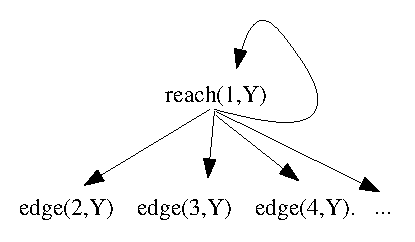
\includegraphics[width=\textwidth]{recursion}
%  \caption{Without \abstraction}
%  \label{fig:minipage1}
\end{minipage}
\quad
\begin{minipage}[b]{0.25\linewidth}
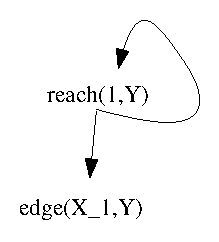
\includegraphics[width=0.5\textwidth]{abs-recursion}
%  \caption{With \abstraction}
%  \label{fig:minipage2}
\end{minipage}
\caption{A left-linear program and schematic IDGs: Left
  without IDG abstraction; Right: with
  IDG abstraction} \label{fig:abstraction}
\end{figure}
%------------------------------------------------------------
Abstracting the {\tt edge/2} predicate has subtle differences from
abstracting tabled subgoals.
%  The implementation of subgoal
%abstraction for tabled subgoals was described in~\cite{RigS13},
As mentioned, the {\tt edge/2} predicate of
Fig.~\ref{fig:abstraction} is not tabled.  Furthermore, the actual
{\tt edge/2} subgoal itself should not be abstracted to depth 0 since
losing the first argument instantiation would prevent the use of
indexing.  Rather, only the IDG's representation of the subgoal
should be abstracted.  Abstraction of dynamic code for
the IDG can be specified via the declaration:
\begin{center}
{\tt :-dynamic edge/2 as incremental, abstract(0)}.
\end{center}

In \version{} dynamic incremental code can be abstracted, but
incremental interned tries (Section~\ref{sec:incr-update-tries})
cannot be.  Also, currently only depth 0 abstraction is supported.

\subsection{Summary and Implementation Status}
%
When using incremental tabling an application will most commonly need
only the default transparent approach, although in special
circumstances eager updating may be desired.  The main design choices
are as usual what to table, and also what dynamic predicates or tries
should be made incremental.  In addition, performance optimizations
may be made through a mixture of subgoal abstraction and dynamic
predicate abstraction.  This optimization can be informed by use of
{\tt statistics/0} which includes summary information about the IDG,
or using the IDG inspection predicates of
Section~\ref{sec:incr-preds1} if more details is needed.

%Thus the user has four choices: tables may be
%updated as soon as the database is changed (e.g., via {\tt
%  incr\_assert/1}); at some point after a series of database changes
%(e.g. via {\tt incr\_assert\_inval/1} and {\tt
%  incr\_table\_update/0}); or lazily whenever a given table is called.
%In addition, if the changes are so massive that there is no point in
%incrementally updating the table, the tables can be abolished so that
%the tables will be reconstructed whenever they are re-queried.

In the current version of XSB, incremental tabling has not yet been
ported to the multi-threaded engine.  In addition, incremental tabling
only works for predicates that use both call and answer variance.
However, incremental tabling does work with for the full well-founded
semantics, for trie indexed dynamic code (in addition to regular
dynamic code) and with interned tries as described in
Section~\ref{sec:incr-update-tries}.  The space reclamation predicates
{\tt abolish\_all\_tables/0}, {\tt abolish\_table\_call/[1,2]} and
{\tt abolish\_table\_pred/[1,2]} can be safely used with incremental
tables.

\subsection{Predicates for Incremental Table Maintenance} \label{sec:incr-preds1}

\paragraph{A Note on Terminology}
%
Suppose {\tt p/1} and {\tt q/1} are incrementally tabled, and that
there is a clause
%
\begin{verbatim}
p(X):- q(X).
\end{verbatim}
%
In this case we say that {\tt p(X)} {\em depends\_on} {\tt q(X)} and
that {\tt q(X)} {\em affects} {\tt p(X)}.  A recursive predicate both
depends on and affects itself.


\paragraph{Declarations} The following directives support incremental
tabling based on changes in dynamic code: 

\index{tabling!opaque}
\index{tabling!declarations}
\begin{description}
\index{tabling!incremental}

\ourstandarditem{table +PredSpecs as incremental}{table/1}{Tabling}
%
is a executable predicate that indicates that each tabled predicate
specified in {\tt PredSpec} is to have its tables maintained
incrementally.  {\tt PredSpec} is a list of skeletons, i.e. open
terms, or {\tt Pred/Arity} specifications~\footnote{No explicit module
  references are allowed.}.  The tables must use call variance and
answer variance and must be compiled and loaded into the
single-threaded engine.  If a predicate is declared with tabling
attributes that are not supported with incremental tabling a
permission error is thrown.  This predicate implies that its arguments
are tabled predicates.  See page \pageref{table-declaration} for
further discussion of tabling options.

We also note that any tabled predicate that is called by a predicate
tabled as incremental must also be tabled as incremental or as opaque.
On the other hand, a dynamic predicate {\tt d/n} that is called by a
predicate tabled as incremental may or may not need to be declared as
incremental.  However if {\tt d/n} is not declared incremental, then
changes to it will not be propagated to incrementally maintained
tables.

\ourstandarditem{dynamic +PredSpecs as incremental}{dynamic/1}{Tabling}
%
is an executable predicate that indicates that each predicate in {\tt
  PredSpecs} is dynamic and used to define an incrementally tabled
predicate and will be updated using {\tt incr\_assert/1} and/or {\tt
  incr\_retractall/1} (or relatives.)  Note that dynamic incremental
predicates cannot themselves be tabled.  This predicate implies that
its arguments are dynamic predicates.  See page
\pageref{dynamic-declaration} for further discussion of dynamic
options.

\ourstandarditem{table +PredSpecs as opaque}{table/1}{Tabling} 
%
is an executable predicate that indicates that each predicate $P$ in
{\tt PredSpecs} is tabled and is used in the definition of some
incrementally tabled predicate but should not be maintained
incrementally.  In this case the system assumes that the programmer
will abolish tables for $P$ in such a way so that re-calling it will
always give semantically correct answers.  In other words, instead of
maintaining information to support incremental table maintenance, the
system re-calls the opaque predicate whenever its results are required
to recompute an answer.  One example of an appropriate use of opaque
is for tabled predicates in a DCG used to parse some string.  Rather
than incrementally maintain all dependencies on all input strings, the
user can declare these intermediate tables as opaque and abolish them
before any call to the DCG.  This predicate implies that its arguments
are tabled predicates.

\end{description}

\paragraph{Basic Incremental Maintenance Predicates}
The following predicates are used to manipulate incrementally
maintained tables:

\begin{description}
\ourrepeatmoditem{incr\_assert(+Clause)}{incr\_assert/1}{increval} 
\ourrepeatmoditem{incr\_assertz(+Clause)}{incr\_assertz/1}{increval}
\ourrepeatmoditem{incr\_asserta(+Clause)}{incr\_asserta/1}{increval}
\ourrepeatmoditem{incr\_retract(+Clause)}{incr\_retract/1}{increval}
\ourmoditem{incr\_retractall(+Term)}{incr\_retractall/1}{increval}
% 
are versions of {\tt assert/1} and other standard Prolog predicates.
They modify dymamic code just as their Prolog counterparts, but they
then invalidate all incrementally maintained tables that depend on
{\tt Clause}.

{\bf Error Cases} are the same as {\tt assert<a/z>/1}, {\tt retract/1}
and {\tt retractall/1} with the additional error condition:

\begin{itemize}
\item The head of the clause {\tt Clause} or the {\tt Term} refers to
  a predicate that is not incremental and dynamic.  
\bi
\item  {\tt type error(dynamic\_incremental, Term)}
\ei
\end{itemize}

\ourrepeatmoditem{incr\_assert\_update(+Clause)}{incr\_assert\_update/1}{increval}
\ourrepeatmoditem{incr\_assertz\_update(+Clause)}{incr\_assertz\_update/1}{increval}
\ourrepeatmoditem{incr\_asserta\_update(+Clause)}{incr\_asserta\_update/1}{increval}\
\ourrepeatmoditem{incr\_retractall\_update(+Clause)}{incr\_retractall\_update/1}{increval}
\ourmoditem{incr\_retract\_update(+Term)}{incr\_retract\_update/1}{increval}
%
are versions of {\tt assert/1} and other standard Prolog predicates.
They modify dymamic code just as their Prolog counterparts, mark any
incrementally maintained tables that depend on the modification as
invalid, then immediately update these tables.
%  The tables may be updated by an
%explicit call to {\tt incr\_table\_update/[0,1,2]}, or the table will
%be dynamically recomputed when a query is made to it.

\ourmoditem{incr\_table\_update}{incr\_table\_update/0}{increval} may
be called after base predicates have been changed (by {\tt
  incr\_assert/1} and/or {\tt incr\_retract/1} or friends).  This
predicate updates all the incrementally maintained tables whose
contents may be affected by those changes to the base predicates.
%This update operation is separated from the operations that change the
%base predicates ({\tt incr\_assert\_inval/1} and {\tt
%  incr\_retractall\_inval/1}) so that a set of base predicate changes
%can be processed all at once, which may be much more efficient that
%updating the tables at every base update.  Beginning with Version
%3.3.7, it is not absolutely necessary to call this predicate, as
%tables will be incrementally updated upon demand.  However, using this
%predicate allows a choice of incurring the cost of update at a time
%other than querying an updated goal.
Explicit update calls only need to be used in special circumstances
(cf. Section~\ref{sec:incr-eager}).

{\bf Error Cases}
\bi
\item A table $T$ that is to be incrementally updated is not yet
  complete.  
\bi
\item 	{\tt permission\_error(update, incomplete\_table Goal)}
\ei
\ei

\ourmoditem{incr\_table\_update(-GoalList)}{incr\_table\_update/1}{increval}
acts as {\tt incr\_table\_update/0} in its action to update the
incrementally maintained tables after changes to base predicates.  It
returns the list of goals whose tables were changed in the update
process.

\ourmoditem{incr\_table\_update(+SkelList,-GoalList)}{incr\_table\_update/2}{increval}
acts as {\tt incr\_table\_update/1} in its action to update
incrementally maintained tables after changes to base predicates.  The
first argument is a list of predicate skeletons (open terms) for
incrementally maintained tables.  The predicate returns in {\tt
  GoalList} a list of goals whose skeletons appear in {\tt SkelList}
and whose tables were changed in the update process.  In this way {\tt
  SkelList} acts as a filter to restrict the goals that are returned
to those of interest.  If {\tt SkelList} is a variable, all affected
goals are returned in {\tt GoalList}.

\ourmoditem{incr\_invalidate\_call(+Goal)}{incr\_invalidate\_call/1}{increval}
is used to directly invalidate a call to an incrementally maintained
table, {\tt Goal}.  A subsequent call to {\tt Goal} will automatically
perform incremental updating for {\tt Goal} along with any tables that
{\tt Goal} depends on that are in need of updating; similarly an
invocation of {\tt incr\_table\_update/[0,1,2]} will cause {\tt Goal}
to be recomputed along with all incrementally maintained tables that
{\tt Goal} affects.  This predicate can be used if a tabled predicate
depends on some external data and not (only) on dynamic incremental
predicates.  For example, if an incrementally maintained predicate
depends on a relation stored in an external relational database
(perhaps accessed through the ODBC interface), then this predicate can
be used to invalidate the table when the external relation changes.
The application programmer must know when the external relation
changes and invoke this predicate as necessary.

{\bf Error Cases}
\bi
\item 	{\tt Goal} is tabled, but not incrementally tabled
\bi
\item 	{\tt permission\_error(invalidate,non-incremental predicate,Goal)}
\ei
\ei

\end{description}

\paragraph{Incremental Maintenance using Interned Tries}
The following predicates are used to modify incremental tries, and can
be freely intermixed with predicates for modifying incremental dynamic
code, as well as with predicates for invalidating or updating tables
(Section~\ref{sec:incr-preds1}).

\begin{description}
\ourmoditem{incr\_trie\_intern(+TrieIdOrAlias,+Term)}{incr\_trie\_intern/2}{intern}
%
is a version of {\tt trie\_intern/2} for tries declared as
incremental.  A call to this predicate interns {\tt Term} in {\tt
  TrieIdOrAlias} and then invalidates all incrementally maintained
tables that depend on this trie.

\ourmoditem{incr\_trie\_uninternall(+TrieIdOrAlias,+Term)}{incr\_trie\_uninternall/2}{intern}
%
is a version of {\tt trie\_unintern/2} for tries declared as
incremental.  A call to this predicate removes all terms unifying with
{\tt Term} in {\tt TrieIdOrAlias} and then invalidates all
incrementally maintained tables that depend on this trie.

\ourmoditem{incr\_trie\_intern\_update(+TrieIdOrAlias,+Term)}
           {incr\_trie\_intern\_update/2}{intern}
%
works for tries declared as incremental in a similar manner as {\tt
  incr\_trie\_intern/2} except that it also immediatesly updates any
affected tables.

\ourmoditem{incr\_trie\_uninternall\_inval(+TrieIdOrAlias,+Term)}
{incr\_trie\_uninternall\_inval/2}{intern}
%
works for tries declared as incremental in a similar manner as {\tt
  incr\_trie\_uninternall/2} except that it also immediately updates
any affected tables.
\end{description}

\index{residual dependency graph}
\index{incremental dependency graph}
\paragraph{Inspecting Dependencies among Incremental Subgoals}
%
% These relations form a labelled directed graph for which the
%nodes are incrementally tabled subgoals present in XSB; a given
%subgoal in the graph may or may not have been completed.  
%Conceptually, there is an edge from $S_1$ to $S_2$ labelled depends
%(affects) if $S_1$ directly depends on (directly affects) $S_2$.  We
%call this graph the {\em incrementally tabled subgoal dependency
%  graph}, or just the incremental dependency graph.  
The predicates in this section allow a user to inspect properties of
IDG that can be useful in debugging, profiling or optimizing a
computation~\footnote{The predicates for traversing the incremental
  dependency graph are somewhat analogous to those for traversing the
  residual dependency graph (Section~\ref{sec:table-inspection}).}.

As explained below, IDG nodes can be accessed via the predicate {\tt
  is\_incremental\_subgoal/1}, while IDG edges can be accessed via
{\tt incr\_directly\_depends/2}.  The predicates {\tt
  get\_incr\_scc/[1,2]} and {\tt get\_incr\_scc\_with\_deps/[3,4]} can
be used to efficiently materialize the dependency graph in Prolog,
including SCC information.

\begin{description}

\ourmoditem{is\_incremental\_subgoal(?Subgoal)}{is\_incremental\_subgoal/1}{increval}
%
This predicate non-deterministically unifies {\tt Subgoal} with
incrementally tabled subgoals that are currently table entries.

\ourmoditem{incr\_directly\_depends(?Goal$_1$,?Goal$_2$)}{incr\_directly\_depends/2}{increval}
accesses the edges of the IDG: the incremental goals (Tables) that
directly depend on or directly affect one another.  At least one of
{\tt Goal$_1$} or {\tt Goal$_2$} must be bound.
\begin{itemize}
\item If {\tt Goal$_1$} is bound, then this predicate will return in
  {\tt Goal$_2$} through backtracking the goals for all incrementally
  maintained tables on which {\tt Goal$_1$} directly depends.
\item If {\tt Goal$_2$} is bound, then it returns in {\tt Goal$_1$}
  through backtracking the goals for all incrementally maintained
  tables that {\tt Goal$_2$} directly affects -- in other words all
  goals that directly depend on {\tt Goal$_2$}.  \ei

{\bf Error Cases}
\bi
\item Neither {\tt Goal$_1$} nor {\tt Goal$_2$} is bound 
\bi
\item 	{\tt instatiation\_error}
\ei
\item {\tt Goal$_1$} and/or {\tt Goal$_2$} is bound, but is not
  incrementally tabled
\bi
\item 	{\tt table\_error}
\ei
\ei

\ourmoditem{incr\_trans\_depends(?Goal$_1$,?Goal$_2$)}{incr\_trans\_depends/2}{increval}
is similar to {\tt incr\_directly\_depends/2} except that it returns
goals according to the transitive closure of the ``directly depends''
relation.  Error conditions are the same as {\tt
  incr\_directly\_depends/2}.

\ourrepeatmoditem{get\_incr\_sccs(?SCCList)}{get\_incr\_sccs/1}{increval}
\ourrepeatmoditem{get\_incr\_sccs\_with\_deps(?SCCList,?DepList)}{get\_incr\_sccs\_with\_deps/2}{increval}
\ourrepeatmoditem{get\_incr\_sccs(+SubgoalList,?SCCList)}{get\_incr\_sccs/2}{increval}
\ourmoditem{get\_incr\_sccs\_with\_deps(+SubgoalList,?SCCList,?DepList)}{get\_incr\_sccs\_with\_deps/3}{increval}
%
Most linear algorithms for SCC detection over a graph use destructive
assignment on a stack to maintain information about the connecteness
of a component; as a result such algorithms are
difficult to write efficiently in Prolog.

{\tt get\_incr\_sccs/1} unifies {\tt SCCList} with SCC information for
the incremental dependency graph that is represented as a list whose
elements are of the form
\begin{center}
{\tt ret(Subgoal,SCC)}.
\end{center}
{\tt SCC} is a numerical index for the SCCs of Subgoal. Two subgoals
are in the same SCC iff they have the same index, however no other
dependency information can be otherwise directly inferred from the
index~\footnote{The actual number for each SCC index depends on how
  the incremental dependency graph happens to be traversed; as a
  result it is best to rely on the index only as a ``generated'' name
  for each SCC.}.

If dependency information is also desired, {\tt
  get\_incr\_scc\_with\_dependencies/2} should be called.  In addition
to the SCC information as above, {\tt DepList} is unified with a list
of dependency terms of the form
\begin{center}
{\tt depends(SCC1,SCC2)}
\end{center}
for each pair {\tt SCC1} and {\tt SCC1} such that some subgoal with
index {\tt SCC1} directly depends on some subgoal with index {\tt
  SCC1}.  If it is necessary to know which subgoal(s) in {\tt SCC1}
directly depends on which subgoal(s) in {\tt SCC2}, the information
can be easily reconstructed using {\tt incr\_directly\_depends/2}
above.  Similarly, {\tt incr\_directly\_depends/2} can be used to
determine the actual edges within a given SCC.

Ordinarily a user will want to see the entire dependency graph and in
such a case the predicates described above should be used.  However,
note that if the dependency graph is the result of several
indepdendent queries it may not be connected.  {\tt get\_incr\_scc/2}
takes as input a list of incremental subgoals, {\tt SubgoalList}.  For
each {\tt Subgoal} in {\tt SubgoalList}, this predicate finds the set
of subgoals connected to {\tt Subgoal} by any mixture of depends and
affects relations, unions these sets together, and finds the SCCs of
all subgoals in the unioned set.

SCC detection is implemented using Tarjan's algorithm~\cite{Tarj72} in
C working directly on XSB's data structures.  The algorithm is
$\cO(|V| + |E|)$ where $|V|$ is the number of vertices and $|E|$ the
number of edges in the dependency graph.  As a result, {\tt
  get\_incr\_sccs/[1,2]} provides an efficient means to materialize the
  high-level topography of the dependency graph~\footnote{Currently,
    the materialization of dependency information between SCCs is
    implemented in a naive manner, so that {\tt
      get\_incr\_sccs\_with\_deps/[2,3]} is $\cO(|V|^2)$.}.

{\bf Error Cases}
\bi
\item {\tt SCCList} contains a predicate that is not tabled
\bi
\item 	{\tt permission\_error}
\ei
\ei
\end{description}



%%% Local Variables: 
%%% mode: latex
%%% TeX-master: "manual1"
%%% End: 

%--------------------------------------------------------------------
